% Options for packages loaded elsewhere
\PassOptionsToPackage{unicode}{hyperref}
\PassOptionsToPackage{hyphens}{url}
%
\documentclass[
  12pt,
]{article}
\title{Effective Pest Treament That Protects Pollinators}
\usepackage{etoolbox}
\makeatletter
\providecommand{\subtitle}[1]{% add subtitle to \maketitle
  \apptocmd{\@title}{\par {\large #1 \par}}{}{}
}
\makeatother
\subtitle{\url{https://github.com/shivanikuckreja/CitrolaKuckrejaSaltman_ENV872_EDA_FinalProject/tree/main/Project}}
\author{Sam Saltman, Shivani Kuckreja, Jessica Citrola}
\date{}

\usepackage{amsmath,amssymb}
\usepackage{lmodern}
\usepackage{iftex}
\ifPDFTeX
  \usepackage[T1]{fontenc}
  \usepackage[utf8]{inputenc}
  \usepackage{textcomp} % provide euro and other symbols
\else % if luatex or xetex
  \usepackage{unicode-math}
  \defaultfontfeatures{Scale=MatchLowercase}
  \defaultfontfeatures[\rmfamily]{Ligatures=TeX,Scale=1}
  \setmainfont[]{Times New Roman}
\fi
% Use upquote if available, for straight quotes in verbatim environments
\IfFileExists{upquote.sty}{\usepackage{upquote}}{}
\IfFileExists{microtype.sty}{% use microtype if available
  \usepackage[]{microtype}
  \UseMicrotypeSet[protrusion]{basicmath} % disable protrusion for tt fonts
}{}
\makeatletter
\@ifundefined{KOMAClassName}{% if non-KOMA class
  \IfFileExists{parskip.sty}{%
    \usepackage{parskip}
  }{% else
    \setlength{\parindent}{0pt}
    \setlength{\parskip}{6pt plus 2pt minus 1pt}}
}{% if KOMA class
  \KOMAoptions{parskip=half}}
\makeatother
\usepackage{xcolor}
\IfFileExists{xurl.sty}{\usepackage{xurl}}{} % add URL line breaks if available
\IfFileExists{bookmark.sty}{\usepackage{bookmark}}{\usepackage{hyperref}}
\hypersetup{
  pdftitle={Effective Pest Treament That Protects Pollinators},
  pdfauthor={Sam Saltman, Shivani Kuckreja, Jessica Citrola},
  hidelinks,
  pdfcreator={LaTeX via pandoc}}
\urlstyle{same} % disable monospaced font for URLs
\usepackage[margin=2.54cm]{geometry}
\usepackage{color}
\usepackage{fancyvrb}
\newcommand{\VerbBar}{|}
\newcommand{\VERB}{\Verb[commandchars=\\\{\}]}
\DefineVerbatimEnvironment{Highlighting}{Verbatim}{commandchars=\\\{\}}
% Add ',fontsize=\small' for more characters per line
\usepackage{framed}
\definecolor{shadecolor}{RGB}{248,248,248}
\newenvironment{Shaded}{\begin{snugshade}}{\end{snugshade}}
\newcommand{\AlertTok}[1]{\textcolor[rgb]{0.94,0.16,0.16}{#1}}
\newcommand{\AnnotationTok}[1]{\textcolor[rgb]{0.56,0.35,0.01}{\textbf{\textit{#1}}}}
\newcommand{\AttributeTok}[1]{\textcolor[rgb]{0.77,0.63,0.00}{#1}}
\newcommand{\BaseNTok}[1]{\textcolor[rgb]{0.00,0.00,0.81}{#1}}
\newcommand{\BuiltInTok}[1]{#1}
\newcommand{\CharTok}[1]{\textcolor[rgb]{0.31,0.60,0.02}{#1}}
\newcommand{\CommentTok}[1]{\textcolor[rgb]{0.56,0.35,0.01}{\textit{#1}}}
\newcommand{\CommentVarTok}[1]{\textcolor[rgb]{0.56,0.35,0.01}{\textbf{\textit{#1}}}}
\newcommand{\ConstantTok}[1]{\textcolor[rgb]{0.00,0.00,0.00}{#1}}
\newcommand{\ControlFlowTok}[1]{\textcolor[rgb]{0.13,0.29,0.53}{\textbf{#1}}}
\newcommand{\DataTypeTok}[1]{\textcolor[rgb]{0.13,0.29,0.53}{#1}}
\newcommand{\DecValTok}[1]{\textcolor[rgb]{0.00,0.00,0.81}{#1}}
\newcommand{\DocumentationTok}[1]{\textcolor[rgb]{0.56,0.35,0.01}{\textbf{\textit{#1}}}}
\newcommand{\ErrorTok}[1]{\textcolor[rgb]{0.64,0.00,0.00}{\textbf{#1}}}
\newcommand{\ExtensionTok}[1]{#1}
\newcommand{\FloatTok}[1]{\textcolor[rgb]{0.00,0.00,0.81}{#1}}
\newcommand{\FunctionTok}[1]{\textcolor[rgb]{0.00,0.00,0.00}{#1}}
\newcommand{\ImportTok}[1]{#1}
\newcommand{\InformationTok}[1]{\textcolor[rgb]{0.56,0.35,0.01}{\textbf{\textit{#1}}}}
\newcommand{\KeywordTok}[1]{\textcolor[rgb]{0.13,0.29,0.53}{\textbf{#1}}}
\newcommand{\NormalTok}[1]{#1}
\newcommand{\OperatorTok}[1]{\textcolor[rgb]{0.81,0.36,0.00}{\textbf{#1}}}
\newcommand{\OtherTok}[1]{\textcolor[rgb]{0.56,0.35,0.01}{#1}}
\newcommand{\PreprocessorTok}[1]{\textcolor[rgb]{0.56,0.35,0.01}{\textit{#1}}}
\newcommand{\RegionMarkerTok}[1]{#1}
\newcommand{\SpecialCharTok}[1]{\textcolor[rgb]{0.00,0.00,0.00}{#1}}
\newcommand{\SpecialStringTok}[1]{\textcolor[rgb]{0.31,0.60,0.02}{#1}}
\newcommand{\StringTok}[1]{\textcolor[rgb]{0.31,0.60,0.02}{#1}}
\newcommand{\VariableTok}[1]{\textcolor[rgb]{0.00,0.00,0.00}{#1}}
\newcommand{\VerbatimStringTok}[1]{\textcolor[rgb]{0.31,0.60,0.02}{#1}}
\newcommand{\WarningTok}[1]{\textcolor[rgb]{0.56,0.35,0.01}{\textbf{\textit{#1}}}}
\usepackage{longtable,booktabs,array}
\usepackage{calc} % for calculating minipage widths
% Correct order of tables after \paragraph or \subparagraph
\usepackage{etoolbox}
\makeatletter
\patchcmd\longtable{\par}{\if@noskipsec\mbox{}\fi\par}{}{}
\makeatother
% Allow footnotes in longtable head/foot
\IfFileExists{footnotehyper.sty}{\usepackage{footnotehyper}}{\usepackage{footnote}}
\makesavenoteenv{longtable}
\usepackage{graphicx}
\makeatletter
\def\maxwidth{\ifdim\Gin@nat@width>\linewidth\linewidth\else\Gin@nat@width\fi}
\def\maxheight{\ifdim\Gin@nat@height>\textheight\textheight\else\Gin@nat@height\fi}
\makeatother
% Scale images if necessary, so that they will not overflow the page
% margins by default, and it is still possible to overwrite the defaults
% using explicit options in \includegraphics[width, height, ...]{}
\setkeys{Gin}{width=\maxwidth,height=\maxheight,keepaspectratio}
% Set default figure placement to htbp
\makeatletter
\def\fps@figure{htbp}
\makeatother
\setlength{\emergencystretch}{3em} % prevent overfull lines
\providecommand{\tightlist}{%
  \setlength{\itemsep}{0pt}\setlength{\parskip}{0pt}}
\setcounter{secnumdepth}{5}
\ifLuaTeX
  \usepackage{selnolig}  % disable illegal ligatures
\fi

\begin{document}
\maketitle

\newpage
\tableofcontents 
\newpage
\listoftables 
\newpage
\listoffigures 
\newpage

\hypertarget{rationale-and-research-questions}{%
\section{Rationale and Research
Questions}\label{rationale-and-research-questions}}

\textbf{Pollination is a critical component of agriculture. Bees are
important pollinators. Our research looks to see if there are exposure
methods and chemicals that do not cause significant harm to bees while
eliminating pests. The goal of our research is to determine potential
treatment methods that reduce pests while having little to no impact on
bees.}

Questions:

\begin{enumerate}
\def\labelenumi{\arabic{enumi}.}
\item
  \emph{Is there an exposure type that has less impact on bees than
  non-bee insects?}
\item
  \emph{Are there chemicals that have a high mortality rate for non-bee
  insects and low rate for bees?}
\end{enumerate}

\newpage

\hypertarget{dataset-information}{%
\section{Dataset Information}\label{dataset-information}}

Data Source: The dataset was pulled from a repository created for
Environmental Data Analytics at Duke University in 2020. The data
collected is from several EPA studies on neonicotinoids and their
effects on insects. The data we will be analyzing is the type of
chemical administered, how it was administered, and how both of these
variables affected insects.

In the wrangling process, we selected the relevant information to our
topic. This includes the chemical type, insect species, lifestage and
age of the species, exposure type and the effect of the exposure.

\begin{Shaded}
\begin{Highlighting}[]
\CommentTok{\#Which exposure types have a significant effect (mortality) on bee species?}
\CommentTok{\#Do not group. Want to see nuances between similar categories }

\NormalTok{BeeMortalityExposureType}\SpecialCharTok{$}\NormalTok{Mortality }\OtherTok{\textless{}{-}} \FunctionTok{ifelse}\NormalTok{(BeeMortalityExposureType}\SpecialCharTok{$}\NormalTok{Effect}\SpecialCharTok{==}\StringTok{"Mortality"}\NormalTok{, }\DecValTok{1}\NormalTok{, }\DecValTok{0}\NormalTok{) }

\CommentTok{\#Making new column categorical}
\NormalTok{BeeMortalityExposureType}\SpecialCharTok{$}\NormalTok{Mortality }\OtherTok{\textless{}{-}} \FunctionTok{as.factor}\NormalTok{(BeeMortalityExposureType}\SpecialCharTok{$}\NormalTok{Mortality)}

\NormalTok{logit }\OtherTok{\textless{}{-}} \FunctionTok{glm}\NormalTok{(Mortality }\SpecialCharTok{\textasciitilde{}}\NormalTok{ Exposure.Type, }\AttributeTok{data =}\NormalTok{ BeeMortalityExposureType, }\AttributeTok{family =} \StringTok{"binomial"}\NormalTok{)}
\FunctionTok{summary}\NormalTok{(logit)}
\end{Highlighting}
\end{Shaded}

\begin{verbatim}
## 
## Call:
## glm(formula = Mortality ~ Exposure.Type, family = "binomial", 
##     data = BeeMortalityExposureType)
## 
## Deviance Residuals: 
##     Min       1Q   Median       3Q      Max  
## -1.4620  -0.7742  -0.7742   1.1774   1.9728  
## 
## Coefficients:
##                                                          Estimate Std. Error
## (Intercept)                                               -0.5306     0.3985
## Exposure.TypeDermal                                       -0.8747     0.5046
## Exposure.TypeDiet, unspecified                             0.5306     0.5836
## Exposure.TypeDirect application                          -16.0354  1696.7344
## Exposure.TypeDrinking water                               17.0967  2399.5448
## Exposure.TypeDropwise                                     17.0967  2399.5448
## Exposure.TypeEnvironmental, unspecified                    0.1252     0.4343
## Exposure.TypeFood                                         -0.5208     0.4052
## Exposure.TypeGround granular                             -16.0354  1073.1091
## Exposure.TypeHand spray                                  -16.0354  1199.7724
## Exposure.TypeMultiple routes between application groups   -1.2611     1.1513
## Exposure.TypeOral via capsule                             17.0967   550.4935
## Exposure.TypeSpray                                         0.2587     0.5186
## Exposure.TypeTopical, general                              1.1787     0.4512
##                                                         z value Pr(>|z|)   
## (Intercept)                                              -1.331    0.183   
## Exposure.TypeDermal                                      -1.734    0.083 . 
## Exposure.TypeDiet, unspecified                            0.909    0.363   
## Exposure.TypeDirect application                          -0.009    0.992   
## Exposure.TypeDrinking water                               0.007    0.994   
## Exposure.TypeDropwise                                     0.007    0.994   
## Exposure.TypeEnvironmental, unspecified                   0.288    0.773   
## Exposure.TypeFood                                        -1.285    0.199   
## Exposure.TypeGround granular                             -0.015    0.988   
## Exposure.TypeHand spray                                  -0.013    0.989   
## Exposure.TypeMultiple routes between application groups  -1.095    0.273   
## Exposure.TypeOral via capsule                             0.031    0.975   
## Exposure.TypeSpray                                        0.499    0.618   
## Exposure.TypeTopical, general                             2.612    0.009 **
## ---
## Signif. codes:  0 '***' 0.001 '**' 0.01 '*' 0.05 '.' 0.1 ' ' 1
## 
## (Dispersion parameter for binomial family taken to be 1)
## 
##     Null deviance: 1757.6  on 1406  degrees of freedom
## Residual deviance: 1621.4  on 1393  degrees of freedom
## AIC: 1649.4
## 
## Number of Fisher Scoring iterations: 15
\end{verbatim}

\begin{Shaded}
\begin{Highlighting}[]
\CommentTok{\#For every one unit change in Topical, the odds of mortality increase by 1.1787. The P value of topical exposure type is 0.009, and is statistically significant.}

\CommentTok{\#Significance: Total topical samples 99 {-} mortality {-} 65}
\CommentTok{\#Additional data collection is needed on: Exposure through soil contact, drinking}
\end{Highlighting}
\end{Shaded}

\begin{Shaded}
\begin{Highlighting}[]
\CommentTok{\#Which exposure types have a significant effect (mortality) on non bee species?}

\NormalTok{NonBeeMortalityExposure}\SpecialCharTok{$}\NormalTok{Mortality }\OtherTok{\textless{}{-}} \FunctionTok{ifelse}\NormalTok{(NonBeeMortalityExposure}\SpecialCharTok{$}\NormalTok{Effect}\SpecialCharTok{==}\StringTok{"Mortality"}\NormalTok{, }\DecValTok{1}\NormalTok{, }\DecValTok{0}\NormalTok{) }

\CommentTok{\#Making new column categorical}
\NormalTok{NonBeeMortalityExposure}\SpecialCharTok{$}\NormalTok{Mortality }\OtherTok{\textless{}{-}} \FunctionTok{as.factor}\NormalTok{(NonBeeMortalityExposure}\SpecialCharTok{$}\NormalTok{Mortality)}

\NormalTok{logit2 }\OtherTok{\textless{}{-}} \FunctionTok{glm}\NormalTok{(Mortality }\SpecialCharTok{\textasciitilde{}}\NormalTok{ Exposure.Type, }\AttributeTok{data =}\NormalTok{ NonBeeMortalityExposure, }\AttributeTok{family =} \StringTok{"binomial"}\NormalTok{)}
\FunctionTok{summary}\NormalTok{(logit2)}
\end{Highlighting}
\end{Shaded}

\begin{verbatim}
## 
## Call:
## glm(formula = Mortality ~ Exposure.Type, family = "binomial", 
##     data = NonBeeMortalityExposure)
## 
## Deviance Residuals: 
##     Min       1Q   Median       3Q      Max  
## -2.2581  -1.0150  -0.1775   1.2435   2.9497  
## 
## Coefficients:
##                                                              Estimate
## (Intercept)                                                    1.1896
## Exposure.TypeDiet, unspecified                                -0.4964
## Exposure.TypeDipped or soaked                                 -1.3921
## Exposure.TypeDirect application                               -1.9780
## Exposure.TypeDrinking water                                   -1.3437
## Exposure.TypeEnvironmental, unspecified                       -1.5843
## Exposure.TypeFilmcoating                                     -18.7557
## Exposure.TypeFoliar spray                                     -5.5269
## Exposure.TypeFood                                             -0.4814
## Exposure.TypeGround granular                                 -18.7557
## Exposure.TypeGround spray                                     -5.3327
## Exposure.TypeHand spray                                       -2.8824
## Exposure.TypeImmersion                                        16.3765
## Exposure.TypeMisted                                          -18.7557
## Exposure.TypeMultiple routes within environmental exposures  -18.7557
## Exposure.TypePresent in soil                                 -18.7557
## Exposure.TypeSpray                                            -2.5710
## Exposure.TypeTopical, general                                  1.2785
## Exposure.TypeWatered                                         -18.7557
##                                                             Std. Error z value
## (Intercept)                                                     0.4317   2.756
## Exposure.TypeDiet, unspecified                                  0.9676  -0.513
## Exposure.TypeDipped or soaked                                   0.4727  -2.945
## Exposure.TypeDirect application                                 0.4774  -4.144
## Exposure.TypeDrinking water                                     0.5840  -2.301
## Exposure.TypeEnvironmental, unspecified                         0.4358  -3.635
## Exposure.TypeFilmcoating                                     3956.1804  -0.005
## Exposure.TypeFoliar spray                                       0.8324  -6.640
## Exposure.TypeFood                                               0.4812  -1.000
## Exposure.TypeGround granular                                  273.0027  -0.069
## Exposure.TypeGround spray                                       1.0965  -4.864
## Exposure.TypeHand spray                                         0.4877  -5.911
## Exposure.TypeImmersion                                       3956.1804   0.004
## Exposure.TypeMisted                                          1398.7210  -0.013
## Exposure.TypeMultiple routes within environmental exposures  2797.4420  -0.007
## Exposure.TypePresent in soil                                 2284.1018  -0.008
## Exposure.TypeSpray                                              0.4592  -5.599
## Exposure.TypeTopical, general                                   0.5430   2.355
## Exposure.TypeWatered                                         1142.0510  -0.016
##                                                             Pr(>|z|)    
## (Intercept)                                                 0.005855 ** 
## Exposure.TypeDiet, unspecified                              0.607926    
## Exposure.TypeDipped or soaked                               0.003227 ** 
## Exposure.TypeDirect application                             3.42e-05 ***
## Exposure.TypeDrinking water                                 0.021404 *  
## Exposure.TypeEnvironmental, unspecified                     0.000278 ***
## Exposure.TypeFilmcoating                                    0.996217    
## Exposure.TypeFoliar spray                                   3.14e-11 ***
## Exposure.TypeFood                                           0.317121    
## Exposure.TypeGround granular                                0.945227    
## Exposure.TypeGround spray                                   1.15e-06 ***
## Exposure.TypeHand spray                                     3.41e-09 ***
## Exposure.TypeImmersion                                      0.996697    
## Exposure.TypeMisted                                         0.989301    
## Exposure.TypeMultiple routes within environmental exposures 0.994651    
## Exposure.TypePresent in soil                                0.993448    
## Exposure.TypeSpray                                          2.16e-08 ***
## Exposure.TypeTopical, general                               0.018538 *  
## Exposure.TypeWatered                                        0.986897    
## ---
## Signif. codes:  0 '***' 0.001 '**' 0.01 '*' 0.05 '.' 0.1 ' ' 1
## 
## (Dispersion parameter for binomial family taken to be 1)
## 
##     Null deviance: 3233.2  on 2528  degrees of freedom
## Residual deviance: 2540.4  on 2510  degrees of freedom
## AIC: 2578.4
## 
## Number of Fisher Scoring iterations: 16
\end{verbatim}

\begin{Shaded}
\begin{Highlighting}[]
\CommentTok{\#Dipped or soaked, Direct application, Environmental{-} unspecified, Foliar spray, Ground spray, Hand spray, Spray, and Topical, general are all significant }

\CommentTok{\#Plenty of samples for non{-}bees {-} correlations  }

\CommentTok{\#Conclusion: Spray could be an effective anthropogenic exposure technique to eliminate pests and preserve bees. Direct application like topical techniques should be avoided as they significantly harm all species. There appears to be environmental exposure types that can promote desired effect as well.}
\end{Highlighting}
\end{Shaded}

\begin{Shaded}
\begin{Highlighting}[]
\CommentTok{\#Which chemical types have a significant effect (mortality) on bee species?}

\NormalTok{logit3 }\OtherTok{\textless{}{-}} \FunctionTok{glm}\NormalTok{(Mortality }\SpecialCharTok{\textasciitilde{}}\NormalTok{ CAS.Number, }\AttributeTok{data =}\NormalTok{ BeeMortalityExposureType, }\AttributeTok{family =} \StringTok{"binomial"}\NormalTok{)}
\FunctionTok{summary}\NormalTok{(logit3)}
\end{Highlighting}
\end{Shaded}

\begin{verbatim}
## 
## Call:
## glm(formula = Mortality ~ CAS.Number, family = "binomial", data = BeeMortalityExposureType)
## 
## Deviance Residuals: 
##     Min       1Q   Median       3Q      Max  
## -1.5453  -0.7585  -0.7585   1.2286   1.7080  
## 
## Coefficients:
##                     Estimate Std. Error z value Pr(>|z|)    
## (Intercept)           0.8329     0.3788   2.199 0.027885 *  
## CAS.Number135410207  -2.0268     0.4568  -4.437 9.10e-06 ***
## CAS.Number138261413  -1.9315     0.3879  -4.979 6.39e-07 ***
## CAS.Number150824478  11.7332   324.7439   0.036 0.971178    
## CAS.Number153719234  -0.9526     0.3993  -2.385 0.017062 *  
## CAS.Number165252700  -1.4276     0.4904  -2.911 0.003599 ** 
## CAS.Number210880925  -1.5066     0.4035  -3.734 0.000189 ***
## ---
## Signif. codes:  0 '***' 0.001 '**' 0.01 '*' 0.05 '.' 0.1 ' ' 1
## 
## (Dispersion parameter for binomial family taken to be 1)
## 
##     Null deviance: 1757.6  on 1406  degrees of freedom
## Residual deviance: 1689.6  on 1400  degrees of freedom
## AIC: 1703.6
## 
## Number of Fisher Scoring iterations: 11
\end{verbatim}

\begin{Shaded}
\begin{Highlighting}[]
 \CommentTok{\#Need more data on 58842209 105843365 and 58842209, 150824478}
 \CommentTok{\# Every other chemical is statistically significant {-} 111988499 135410207 138261413  153719234 165252700 210880925 }
\end{Highlighting}
\end{Shaded}

\begin{Shaded}
\begin{Highlighting}[]
\CommentTok{\#Which exposure types have a significant effect (mortality) on non bee species?}

\NormalTok{logit4 }\OtherTok{\textless{}{-}} \FunctionTok{glm}\NormalTok{(Mortality }\SpecialCharTok{\textasciitilde{}}\NormalTok{ CAS.Number, }\AttributeTok{data =}\NormalTok{ NonBeeMortalityExposure, }\AttributeTok{family =} \StringTok{"binomial"}\NormalTok{)}
\FunctionTok{summary}\NormalTok{(logit4)}
\end{Highlighting}
\end{Shaded}

\begin{verbatim}
## 
## Call:
## glm(formula = Mortality ~ CAS.Number, family = "binomial", data = NonBeeMortalityExposure)
## 
## Deviance Residuals: 
##     Min       1Q   Median       3Q      Max  
## -1.5928  -0.8379  -0.8379   1.2907   1.9027  
## 
## Coefficients:
##                       Estimate Std. Error z value Pr(>|z|)
## (Intercept)          1.557e+01  4.602e+02   0.034    0.973
## CAS.Number105843365  1.448e-09  6.509e+02   0.000    1.000
## CAS.Number111988499 -1.507e+01  4.602e+02  -0.033    0.974
## CAS.Number135410207 -1.583e+01  4.602e+02  -0.034    0.973
## CAS.Number138261413 -1.643e+01  4.602e+02  -0.036    0.972
## CAS.Number150824478 -1.463e+01  4.602e+02  -0.032    0.975
## CAS.Number153719234 -1.615e+01  4.602e+02  -0.035    0.972
## CAS.Number165252700 -1.580e+01  4.602e+02  -0.034    0.973
## CAS.Number210880925 -1.720e+01  4.602e+02  -0.037    0.970
## 
## (Dispersion parameter for binomial family taken to be 1)
## 
##     Null deviance: 3233.2  on 2528  degrees of freedom
## Residual deviance: 3091.8  on 2520  degrees of freedom
## AIC: 3109.8
## 
## Number of Fisher Scoring iterations: 14
\end{verbatim}

\begin{Shaded}
\begin{Highlighting}[]
 \CommentTok{\#There is no chemical that is effective at eliminating all non{-}bee species. }
 \CommentTok{\#Conclusion {-} exposure mechanism of chemical is a more reliable factor at understanding mortality than chemical itself. Bees do not respond well to any of the adminstered chemicals. Any treatment should focus on using the chemicals in ways that are ineffective at exposing bees and effective at exposing nonbees}
\end{Highlighting}
\end{Shaded}

\begin{Shaded}
\begin{Highlighting}[]
\NormalTok{logit5 }\OtherTok{\textless{}{-}} \FunctionTok{glm}\NormalTok{(Mortality }\SpecialCharTok{\textasciitilde{}}\NormalTok{ CAS.Number }\SpecialCharTok{*}\NormalTok{ Exposure.Type, }\AttributeTok{data =}\NormalTok{ NonBeeMortalityExposure, }\AttributeTok{family =} \StringTok{"binomial"}\NormalTok{)}
\end{Highlighting}
\end{Shaded}

\begin{verbatim}
## Warning: glm.fit: algorithm did not converge
\end{verbatim}

\begin{verbatim}
## Warning: glm.fit: fitted probabilities numerically 0 or 1 occurred
\end{verbatim}

\begin{Shaded}
\begin{Highlighting}[]
\FunctionTok{summary}\NormalTok{(logit5)}
\end{Highlighting}
\end{Shaded}

\begin{verbatim}
## 
## Call:
## glm(formula = Mortality ~ CAS.Number * Exposure.Type, family = "binomial", 
##     data = NonBeeMortalityExposure)
## 
## Deviance Residuals: 
##     Min       1Q   Median       3Q      Max  
## -2.4230  -0.9870  -0.1678   0.9091   2.9223  
## 
## Coefficients: (92 not defined because of singularities)
##                                                                                   Estimate
## (Intercept)                                                                      1.790e+11
## CAS.Number105843365                                                              4.504e+15
## CAS.Number111988499                                                             -7.211e+12
## CAS.Number135410207                                                              1.809e+11
## CAS.Number138261413                                                             -1.790e+11
## CAS.Number150824478                                                             -3.417e+13
## CAS.Number153719234                                                             -1.790e+11
## CAS.Number165252700                                                             -1.790e+11
## CAS.Number210880925                                                             -1.250e+01
## Exposure.TypeDiet, unspecified                                                   6.461e+12
## Exposure.TypeDipped or soaked                                                   -2.750e+01
## Exposure.TypeDirect application                                                 -1.790e+11
## Exposure.TypeDrinking water                                                     -7.728e+11
## Exposure.TypeEnvironmental, unspecified                                         -1.790e+11
## Exposure.TypeFilmcoating                                                        -2.712e+01
## Exposure.TypeFoliar spray                                                       -5.264e+12
## Exposure.TypeFood                                                               -1.790e+11
## Exposure.TypeGround granular                                                    -4.871e+01
## Exposure.TypeGround spray                                                       -2.869e+01
## Exposure.TypeHand spray                                                         -1.790e+11
## Exposure.TypeImmersion                                                           4.344e+01
## Exposure.TypeMisted                                                             -5.392e+01
## Exposure.TypeMultiple routes within environmental exposures                     -3.418e+01
## Exposure.TypePresent in soil                                                    -2.869e+01
## Exposure.TypeSpray                                                              -1.003e+12
## Exposure.TypeTopical, general                                                    1.758e+13
## Exposure.TypeWatered                                                            -4.504e+15
## CAS.Number105843365:Exposure.TypeDiet, unspecified                                      NA
## CAS.Number111988499:Exposure.TypeDiet, unspecified                                      NA
## CAS.Number135410207:Exposure.TypeDiet, unspecified                               4.497e+15
## CAS.Number138261413:Exposure.TypeDiet, unspecified                              -6.461e+12
## CAS.Number150824478:Exposure.TypeDiet, unspecified                               4.531e+15
## CAS.Number153719234:Exposure.TypeDiet, unspecified                                      NA
## CAS.Number165252700:Exposure.TypeDiet, unspecified                                      NA
## CAS.Number210880925:Exposure.TypeDiet, unspecified                               4.497e+15
## CAS.Number105843365:Exposure.TypeDipped or soaked                                       NA
## CAS.Number111988499:Exposure.TypeDipped or soaked                               -4.497e+15
## CAS.Number135410207:Exposure.TypeDipped or soaked                               -3.599e+11
## CAS.Number138261413:Exposure.TypeDipped or soaked                                2.709e+01
## CAS.Number150824478:Exposure.TypeDipped or soaked                                3.399e+13
## CAS.Number153719234:Exposure.TypeDipped or soaked                               -1.000e+00
## CAS.Number165252700:Exposure.TypeDipped or soaked                                       NA
## CAS.Number210880925:Exposure.TypeDipped or soaked                                       NA
## CAS.Number105843365:Exposure.TypeDirect application                                     NA
## CAS.Number111988499:Exposure.TypeDirect application                                     NA
## CAS.Number135410207:Exposure.TypeDirect application                             -1.809e+11
## CAS.Number138261413:Exposure.TypeDirect application                              1.790e+11
## CAS.Number150824478:Exposure.TypeDirect application                                     NA
## CAS.Number153719234:Exposure.TypeDirect application                              1.790e+11
## CAS.Number165252700:Exposure.TypeDirect application                              1.790e+11
## CAS.Number210880925:Exposure.TypeDirect application                                     NA
## CAS.Number105843365:Exposure.TypeDrinking water                                         NA
## CAS.Number111988499:Exposure.TypeDrinking water                                         NA
## CAS.Number135410207:Exposure.TypeDrinking water                                         NA
## CAS.Number138261413:Exposure.TypeDrinking water                                  7.728e+11
## CAS.Number150824478:Exposure.TypeDrinking water                                         NA
## CAS.Number153719234:Exposure.TypeDrinking water                                 -4.503e+15
## CAS.Number165252700:Exposure.TypeDrinking water                                         NA
## CAS.Number210880925:Exposure.TypeDrinking water                                         NA
## CAS.Number105843365:Exposure.TypeEnvironmental, unspecified                             NA
## CAS.Number111988499:Exposure.TypeEnvironmental, unspecified                      7.211e+12
## CAS.Number135410207:Exposure.TypeEnvironmental, unspecified                     -1.809e+11
## CAS.Number138261413:Exposure.TypeEnvironmental, unspecified                      1.790e+11
## CAS.Number150824478:Exposure.TypeEnvironmental, unspecified                      3.417e+13
## CAS.Number153719234:Exposure.TypeEnvironmental, unspecified                      1.790e+11
## CAS.Number165252700:Exposure.TypeEnvironmental, unspecified                      1.790e+11
## CAS.Number210880925:Exposure.TypeEnvironmental, unspecified                             NA
## CAS.Number105843365:Exposure.TypeFilmcoating                                            NA
## CAS.Number111988499:Exposure.TypeFilmcoating                                            NA
## CAS.Number135410207:Exposure.TypeFilmcoating                                            NA
## CAS.Number138261413:Exposure.TypeFilmcoating                                            NA
## CAS.Number150824478:Exposure.TypeFilmcoating                                            NA
## CAS.Number153719234:Exposure.TypeFilmcoating                                            NA
## CAS.Number165252700:Exposure.TypeFilmcoating                                            NA
## CAS.Number210880925:Exposure.TypeFilmcoating                                            NA
## CAS.Number105843365:Exposure.TypeFoliar spray                                           NA
## CAS.Number111988499:Exposure.TypeFoliar spray                                           NA
## CAS.Number135410207:Exposure.TypeFoliar spray                                    4.904e+12
## CAS.Number138261413:Exposure.TypeFoliar spray                                    5.264e+12
## CAS.Number150824478:Exposure.TypeFoliar spray                                           NA
## CAS.Number153719234:Exposure.TypeFoliar spray                                    5.264e+12
## CAS.Number165252700:Exposure.TypeFoliar spray                                    5.264e+12
## CAS.Number210880925:Exposure.TypeFoliar spray                                    5.085e+12
## CAS.Number105843365:Exposure.TypeFood                                                   NA
## CAS.Number111988499:Exposure.TypeFood                                                   NA
## CAS.Number135410207:Exposure.TypeFood                                                   NA
## CAS.Number138261413:Exposure.TypeFood                                            1.790e+11
## CAS.Number150824478:Exposure.TypeFood                                            3.417e+13
## CAS.Number153719234:Exposure.TypeFood                                            1.790e+11
## CAS.Number165252700:Exposure.TypeFood                                            1.790e+11
## CAS.Number210880925:Exposure.TypeFood                                                   NA
## CAS.Number105843365:Exposure.TypeGround granular                                        NA
## CAS.Number111988499:Exposure.TypeGround granular                                        NA
## CAS.Number135410207:Exposure.TypeGround granular                                        NA
## CAS.Number138261413:Exposure.TypeGround granular                                 2.000e+01
## CAS.Number150824478:Exposure.TypeGround granular                                        NA
## CAS.Number153719234:Exposure.TypeGround granular                                        NA
## CAS.Number165252700:Exposure.TypeGround granular                                        NA
## CAS.Number210880925:Exposure.TypeGround granular                                        NA
## CAS.Number105843365:Exposure.TypeGround spray                                           NA
## CAS.Number111988499:Exposure.TypeGround spray                                           NA
## CAS.Number135410207:Exposure.TypeGround spray                                   -3.599e+11
## CAS.Number138261413:Exposure.TypeGround spray                                   -4.504e+15
## CAS.Number150824478:Exposure.TypeGround spray                                           NA
## CAS.Number153719234:Exposure.TypeGround spray                                   -1.785e+01
## CAS.Number165252700:Exposure.TypeGround spray                                           NA
## CAS.Number210880925:Exposure.TypeGround spray                                           NA
## CAS.Number105843365:Exposure.TypeHand spray                                             NA
## CAS.Number111988499:Exposure.TypeHand spray                                      7.211e+12
## CAS.Number135410207:Exposure.TypeHand spray                                     -1.809e+11
## CAS.Number138261413:Exposure.TypeHand spray                                      1.790e+11
## CAS.Number150824478:Exposure.TypeHand spray                                             NA
## CAS.Number153719234:Exposure.TypeHand spray                                      1.790e+11
## CAS.Number165252700:Exposure.TypeHand spray                                      1.790e+11
## CAS.Number210880925:Exposure.TypeHand spray                                             NA
## CAS.Number105843365:Exposure.TypeImmersion                                              NA
## CAS.Number111988499:Exposure.TypeImmersion                                              NA
## CAS.Number135410207:Exposure.TypeImmersion                                              NA
## CAS.Number138261413:Exposure.TypeImmersion                                              NA
## CAS.Number150824478:Exposure.TypeImmersion                                              NA
## CAS.Number153719234:Exposure.TypeImmersion                                              NA
## CAS.Number165252700:Exposure.TypeImmersion                                              NA
## CAS.Number210880925:Exposure.TypeImmersion                                              NA
## CAS.Number105843365:Exposure.TypeMisted                                                 NA
## CAS.Number111988499:Exposure.TypeMisted                                                 NA
## CAS.Number135410207:Exposure.TypeMisted                                         -3.599e+11
## CAS.Number138261413:Exposure.TypeMisted                                                 NA
## CAS.Number150824478:Exposure.TypeMisted                                                 NA
## CAS.Number153719234:Exposure.TypeMisted                                                 NA
## CAS.Number165252700:Exposure.TypeMisted                                                 NA
## CAS.Number210880925:Exposure.TypeMisted                                                 NA
## CAS.Number105843365:Exposure.TypeMultiple routes within environmental exposures         NA
## CAS.Number111988499:Exposure.TypeMultiple routes within environmental exposures         NA
## CAS.Number135410207:Exposure.TypeMultiple routes within environmental exposures         NA
## CAS.Number138261413:Exposure.TypeMultiple routes within environmental exposures         NA
## CAS.Number150824478:Exposure.TypeMultiple routes within environmental exposures         NA
## CAS.Number153719234:Exposure.TypeMultiple routes within environmental exposures         NA
## CAS.Number165252700:Exposure.TypeMultiple routes within environmental exposures         NA
## CAS.Number210880925:Exposure.TypeMultiple routes within environmental exposures         NA
## CAS.Number105843365:Exposure.TypePresent in soil                                        NA
## CAS.Number111988499:Exposure.TypePresent in soil                                        NA
## CAS.Number135410207:Exposure.TypePresent in soil                                        NA
## CAS.Number138261413:Exposure.TypePresent in soil                                        NA
## CAS.Number150824478:Exposure.TypePresent in soil                                        NA
## CAS.Number153719234:Exposure.TypePresent in soil                                        NA
## CAS.Number165252700:Exposure.TypePresent in soil                                        NA
## CAS.Number210880925:Exposure.TypePresent in soil                                        NA
## CAS.Number105843365:Exposure.TypeSpray                                                  NA
## CAS.Number111988499:Exposure.TypeSpray                                           8.035e+12
## CAS.Number135410207:Exposure.TypeSpray                                           6.427e+11
## CAS.Number138261413:Exposure.TypeSpray                                           1.003e+12
## CAS.Number150824478:Exposure.TypeSpray                                                  NA
## CAS.Number153719234:Exposure.TypeSpray                                           1.003e+12
## CAS.Number165252700:Exposure.TypeSpray                                           1.003e+12
## CAS.Number210880925:Exposure.TypeSpray                                           8.236e+11
## CAS.Number105843365:Exposure.TypeTopical, general                                       NA
## CAS.Number111988499:Exposure.TypeTopical, general                                4.493e+15
## CAS.Number135410207:Exposure.TypeTopical, general                               -1.794e+13
## CAS.Number138261413:Exposure.TypeTopical, general                               -1.758e+13
## CAS.Number150824478:Exposure.TypeTopical, general                                       NA
## CAS.Number153719234:Exposure.TypeTopical, general                               -1.758e+13
## CAS.Number165252700:Exposure.TypeTopical, general                               -1.758e+13
## CAS.Number210880925:Exposure.TypeTopical, general                                       NA
## CAS.Number105843365:Exposure.TypeWatered                                                NA
## CAS.Number111988499:Exposure.TypeWatered                                                NA
## CAS.Number135410207:Exposure.TypeWatered                                                NA
## CAS.Number138261413:Exposure.TypeWatered                                        -4.066e+04
## CAS.Number150824478:Exposure.TypeWatered                                                NA
## CAS.Number153719234:Exposure.TypeWatered                                                NA
## CAS.Number165252700:Exposure.TypeWatered                                                NA
## CAS.Number210880925:Exposure.TypeWatered                                                NA
##                                                                                 Std. Error
## (Intercept)                                                                      1.603e+12
## CAS.Number105843365                                                              2.122e+07
## CAS.Number111988499                                                              1.121e+13
## CAS.Number135410207                                                              2.447e+12
## CAS.Number138261413                                                              1.603e+12
## CAS.Number150824478                                                              8.835e+13
## CAS.Number153719234                                                              1.603e+12
## CAS.Number165252700                                                              1.603e+12
## CAS.Number210880925                                                              1.541e+01
## Exposure.TypeDiet, unspecified                                                   1.338e+14
## Exposure.TypeDipped or soaked                                                    1.490e+05
## Exposure.TypeDirect application                                                  1.603e+12
## Exposure.TypeDrinking water                                                      1.927e+13
## Exposure.TypeEnvironmental, unspecified                                          1.603e+12
## Exposure.TypeFilmcoating                                                         4.164e+05
## Exposure.TypeFoliar spray                                                        1.936e+14
## Exposure.TypeFood                                                                1.603e+12
## Exposure.TypeGround granular                                                     6.438e+05
## Exposure.TypeGround spray                                                        1.490e+05
## Exposure.TypeHand spray                                                          1.603e+12
## Exposure.TypeImmersion                                                           6.711e+07
## Exposure.TypeMisted                                                              7.799e+05
## Exposure.TypeMultiple routes within environmental exposures                      4.745e+07
## Exposure.TypePresent in soil                                                     3.214e+05
## Exposure.TypeSpray                                                               6.498e+12
## Exposure.TypeTopical, general                                                    2.162e+13
## Exposure.TypeWatered                                                             4.746e+07
## CAS.Number105843365:Exposure.TypeDiet, unspecified                                      NA
## CAS.Number111988499:Exposure.TypeDiet, unspecified                                      NA
## CAS.Number135410207:Exposure.TypeDiet, unspecified                               1.337e+14
## CAS.Number138261413:Exposure.TypeDiet, unspecified                               1.338e+14
## CAS.Number150824478:Exposure.TypeDiet, unspecified                               1.630e+14
## CAS.Number153719234:Exposure.TypeDiet, unspecified                                      NA
## CAS.Number165252700:Exposure.TypeDiet, unspecified                                      NA
## CAS.Number210880925:Exposure.TypeDiet, unspecified                               1.339e+14
## CAS.Number105843365:Exposure.TypeDipped or soaked                                       NA
## CAS.Number111988499:Exposure.TypeDipped or soaked                                1.110e+13
## CAS.Number135410207:Exposure.TypeDipped or soaked                                2.717e+12
## CAS.Number138261413:Exposure.TypeDipped or soaked                                1.490e+05
## CAS.Number150824478:Exposure.TypeDipped or soaked                                8.861e+13
## CAS.Number153719234:Exposure.TypeDipped or soaked                                6.606e+05
## CAS.Number165252700:Exposure.TypeDipped or soaked                                       NA
## CAS.Number210880925:Exposure.TypeDipped or soaked                                       NA
## CAS.Number105843365:Exposure.TypeDirect application                                     NA
## CAS.Number111988499:Exposure.TypeDirect application                                     NA
## CAS.Number135410207:Exposure.TypeDirect application                              2.447e+12
## CAS.Number138261413:Exposure.TypeDirect application                              1.603e+12
## CAS.Number150824478:Exposure.TypeDirect application                                     NA
## CAS.Number153719234:Exposure.TypeDirect application                              1.603e+12
## CAS.Number165252700:Exposure.TypeDirect application                              1.603e+12
## CAS.Number210880925:Exposure.TypeDirect application                                     NA
## CAS.Number105843365:Exposure.TypeDrinking water                                         NA
## CAS.Number111988499:Exposure.TypeDrinking water                                         NA
## CAS.Number135410207:Exposure.TypeDrinking water                                         NA
## CAS.Number138261413:Exposure.TypeDrinking water                                  1.927e+13
## CAS.Number150824478:Exposure.TypeDrinking water                                         NA
## CAS.Number153719234:Exposure.TypeDrinking water                                  1.927e+13
## CAS.Number165252700:Exposure.TypeDrinking water                                         NA
## CAS.Number210880925:Exposure.TypeDrinking water                                         NA
## CAS.Number105843365:Exposure.TypeEnvironmental, unspecified                             NA
## CAS.Number111988499:Exposure.TypeEnvironmental, unspecified                      1.121e+13
## CAS.Number135410207:Exposure.TypeEnvironmental, unspecified                      2.447e+12
## CAS.Number138261413:Exposure.TypeEnvironmental, unspecified                      1.603e+12
## CAS.Number150824478:Exposure.TypeEnvironmental, unspecified                      8.835e+13
## CAS.Number153719234:Exposure.TypeEnvironmental, unspecified                      1.603e+12
## CAS.Number165252700:Exposure.TypeEnvironmental, unspecified                      1.603e+12
## CAS.Number210880925:Exposure.TypeEnvironmental, unspecified                             NA
## CAS.Number105843365:Exposure.TypeFilmcoating                                            NA
## CAS.Number111988499:Exposure.TypeFilmcoating                                            NA
## CAS.Number135410207:Exposure.TypeFilmcoating                                            NA
## CAS.Number138261413:Exposure.TypeFilmcoating                                            NA
## CAS.Number150824478:Exposure.TypeFilmcoating                                            NA
## CAS.Number153719234:Exposure.TypeFilmcoating                                            NA
## CAS.Number165252700:Exposure.TypeFilmcoating                                            NA
## CAS.Number210880925:Exposure.TypeFilmcoating                                            NA
## CAS.Number105843365:Exposure.TypeFoliar spray                                           NA
## CAS.Number111988499:Exposure.TypeFoliar spray                                           NA
## CAS.Number135410207:Exposure.TypeFoliar spray                                    1.944e+14
## CAS.Number138261413:Exposure.TypeFoliar spray                                    1.936e+14
## CAS.Number150824478:Exposure.TypeFoliar spray                                           NA
## CAS.Number153719234:Exposure.TypeFoliar spray                                    1.936e+14
## CAS.Number165252700:Exposure.TypeFoliar spray                                    1.936e+14
## CAS.Number210880925:Exposure.TypeFoliar spray                                    1.936e+14
## CAS.Number105843365:Exposure.TypeFood                                                   NA
## CAS.Number111988499:Exposure.TypeFood                                                   NA
## CAS.Number135410207:Exposure.TypeFood                                                   NA
## CAS.Number138261413:Exposure.TypeFood                                            1.603e+12
## CAS.Number150824478:Exposure.TypeFood                                            8.835e+13
## CAS.Number153719234:Exposure.TypeFood                                            1.603e+12
## CAS.Number165252700:Exposure.TypeFood                                            1.603e+12
## CAS.Number210880925:Exposure.TypeFood                                                   NA
## CAS.Number105843365:Exposure.TypeGround granular                                        NA
## CAS.Number111988499:Exposure.TypeGround granular                                        NA
## CAS.Number135410207:Exposure.TypeGround granular                                        NA
## CAS.Number138261413:Exposure.TypeGround granular                                 6.444e+05
## CAS.Number150824478:Exposure.TypeGround granular                                        NA
## CAS.Number153719234:Exposure.TypeGround granular                                        NA
## CAS.Number165252700:Exposure.TypeGround granular                                        NA
## CAS.Number210880925:Exposure.TypeGround granular                                        NA
## CAS.Number105843365:Exposure.TypeGround spray                                           NA
## CAS.Number111988499:Exposure.TypeGround spray                                           NA
## CAS.Number135410207:Exposure.TypeGround spray                                    2.717e+12
## CAS.Number138261413:Exposure.TypeGround spray                                    8.969e+06
## CAS.Number150824478:Exposure.TypeGround spray                                           NA
## CAS.Number153719234:Exposure.TypeGround spray                                    6.606e+05
## CAS.Number165252700:Exposure.TypeGround spray                                           NA
## CAS.Number210880925:Exposure.TypeGround spray                                           NA
## CAS.Number105843365:Exposure.TypeHand spray                                             NA
## CAS.Number111988499:Exposure.TypeHand spray                                      1.121e+13
## CAS.Number135410207:Exposure.TypeHand spray                                      2.447e+12
## CAS.Number138261413:Exposure.TypeHand spray                                      1.603e+12
## CAS.Number150824478:Exposure.TypeHand spray                                             NA
## CAS.Number153719234:Exposure.TypeHand spray                                      1.603e+12
## CAS.Number165252700:Exposure.TypeHand spray                                      1.603e+12
## CAS.Number210880925:Exposure.TypeHand spray                                             NA
## CAS.Number105843365:Exposure.TypeImmersion                                              NA
## CAS.Number111988499:Exposure.TypeImmersion                                              NA
## CAS.Number135410207:Exposure.TypeImmersion                                              NA
## CAS.Number138261413:Exposure.TypeImmersion                                              NA
## CAS.Number150824478:Exposure.TypeImmersion                                              NA
## CAS.Number153719234:Exposure.TypeImmersion                                              NA
## CAS.Number165252700:Exposure.TypeImmersion                                              NA
## CAS.Number210880925:Exposure.TypeImmersion                                              NA
## CAS.Number105843365:Exposure.TypeMisted                                                 NA
## CAS.Number111988499:Exposure.TypeMisted                                                 NA
## CAS.Number135410207:Exposure.TypeMisted                                          2.717e+12
## CAS.Number138261413:Exposure.TypeMisted                                                 NA
## CAS.Number150824478:Exposure.TypeMisted                                                 NA
## CAS.Number153719234:Exposure.TypeMisted                                                 NA
## CAS.Number165252700:Exposure.TypeMisted                                                 NA
## CAS.Number210880925:Exposure.TypeMisted                                                 NA
## CAS.Number105843365:Exposure.TypeMultiple routes within environmental exposures         NA
## CAS.Number111988499:Exposure.TypeMultiple routes within environmental exposures         NA
## CAS.Number135410207:Exposure.TypeMultiple routes within environmental exposures         NA
## CAS.Number138261413:Exposure.TypeMultiple routes within environmental exposures         NA
## CAS.Number150824478:Exposure.TypeMultiple routes within environmental exposures         NA
## CAS.Number153719234:Exposure.TypeMultiple routes within environmental exposures         NA
## CAS.Number165252700:Exposure.TypeMultiple routes within environmental exposures         NA
## CAS.Number210880925:Exposure.TypeMultiple routes within environmental exposures         NA
## CAS.Number105843365:Exposure.TypePresent in soil                                        NA
## CAS.Number111988499:Exposure.TypePresent in soil                                        NA
## CAS.Number135410207:Exposure.TypePresent in soil                                        NA
## CAS.Number138261413:Exposure.TypePresent in soil                                        NA
## CAS.Number150824478:Exposure.TypePresent in soil                                        NA
## CAS.Number153719234:Exposure.TypePresent in soil                                        NA
## CAS.Number165252700:Exposure.TypePresent in soil                                        NA
## CAS.Number210880925:Exposure.TypePresent in soil                                        NA
## CAS.Number105843365:Exposure.TypeSpray                                                  NA
## CAS.Number111988499:Exposure.TypeSpray                                           9.655e+12
## CAS.Number135410207:Exposure.TypeSpray                                           5.963e+12
## CAS.Number138261413:Exposure.TypeSpray                                           6.498e+12
## CAS.Number150824478:Exposure.TypeSpray                                                  NA
## CAS.Number153719234:Exposure.TypeSpray                                           6.498e+12
## CAS.Number165252700:Exposure.TypeSpray                                           6.498e+12
## CAS.Number210880925:Exposure.TypeSpray                                           6.676e+12
## CAS.Number105843365:Exposure.TypeTopical, general                                       NA
## CAS.Number111988499:Exposure.TypeTopical, general                                2.286e+13
## CAS.Number135410207:Exposure.TypeTopical, general                                2.190e+13
## CAS.Number138261413:Exposure.TypeTopical, general                                2.162e+13
## CAS.Number150824478:Exposure.TypeTopical, general                                       NA
## CAS.Number153719234:Exposure.TypeTopical, general                                2.162e+13
## CAS.Number165252700:Exposure.TypeTopical, general                                2.162e+13
## CAS.Number210880925:Exposure.TypeTopical, general                                       NA
## CAS.Number105843365:Exposure.TypeWatered                                                NA
## CAS.Number111988499:Exposure.TypeWatered                                                NA
## CAS.Number135410207:Exposure.TypeWatered                                                NA
## CAS.Number138261413:Exposure.TypeWatered                                         5.199e+07
## CAS.Number150824478:Exposure.TypeWatered                                                NA
## CAS.Number153719234:Exposure.TypeWatered                                                NA
## CAS.Number165252700:Exposure.TypeWatered                                                NA
## CAS.Number210880925:Exposure.TypeWatered                                                NA
##                                                                                    z value
## (Intercept)                                                                      1.120e-01
## CAS.Number105843365                                                              2.122e+08
## CAS.Number111988499                                                             -6.430e-01
## CAS.Number135410207                                                              7.400e-02
## CAS.Number138261413                                                             -1.120e-01
## CAS.Number150824478                                                             -3.870e-01
## CAS.Number153719234                                                             -1.120e-01
## CAS.Number165252700                                                             -1.120e-01
## CAS.Number210880925                                                             -8.110e-01
## Exposure.TypeDiet, unspecified                                                   4.800e-02
## Exposure.TypeDipped or soaked                                                    0.000e+00
## Exposure.TypeDirect application                                                 -1.120e-01
## Exposure.TypeDrinking water                                                     -4.000e-02
## Exposure.TypeEnvironmental, unspecified                                         -1.120e-01
## Exposure.TypeFilmcoating                                                         0.000e+00
## Exposure.TypeFoliar spray                                                       -2.700e-02
## Exposure.TypeFood                                                               -1.120e-01
## Exposure.TypeGround granular                                                     0.000e+00
## Exposure.TypeGround spray                                                        0.000e+00
## Exposure.TypeHand spray                                                         -1.120e-01
## Exposure.TypeImmersion                                                           0.000e+00
## Exposure.TypeMisted                                                              0.000e+00
## Exposure.TypeMultiple routes within environmental exposures                      0.000e+00
## Exposure.TypePresent in soil                                                     0.000e+00
## Exposure.TypeSpray                                                              -1.540e-01
## Exposure.TypeTopical, general                                                    8.130e-01
## Exposure.TypeWatered                                                            -9.489e+07
## CAS.Number105843365:Exposure.TypeDiet, unspecified                                      NA
## CAS.Number111988499:Exposure.TypeDiet, unspecified                                      NA
## CAS.Number135410207:Exposure.TypeDiet, unspecified                               3.362e+01
## CAS.Number138261413:Exposure.TypeDiet, unspecified                              -4.800e-02
## CAS.Number150824478:Exposure.TypeDiet, unspecified                               2.779e+01
## CAS.Number153719234:Exposure.TypeDiet, unspecified                                      NA
## CAS.Number165252700:Exposure.TypeDiet, unspecified                                      NA
## CAS.Number210880925:Exposure.TypeDiet, unspecified                               3.359e+01
## CAS.Number105843365:Exposure.TypeDipped or soaked                                       NA
## CAS.Number111988499:Exposure.TypeDipped or soaked                               -4.053e+02
## CAS.Number135410207:Exposure.TypeDipped or soaked                               -1.320e-01
## CAS.Number138261413:Exposure.TypeDipped or soaked                                0.000e+00
## CAS.Number150824478:Exposure.TypeDipped or soaked                                3.840e-01
## CAS.Number153719234:Exposure.TypeDipped or soaked                                0.000e+00
## CAS.Number165252700:Exposure.TypeDipped or soaked                                       NA
## CAS.Number210880925:Exposure.TypeDipped or soaked                                       NA
## CAS.Number105843365:Exposure.TypeDirect application                                     NA
## CAS.Number111988499:Exposure.TypeDirect application                                     NA
## CAS.Number135410207:Exposure.TypeDirect application                             -7.400e-02
## CAS.Number138261413:Exposure.TypeDirect application                              1.120e-01
## CAS.Number150824478:Exposure.TypeDirect application                                     NA
## CAS.Number153719234:Exposure.TypeDirect application                              1.120e-01
## CAS.Number165252700:Exposure.TypeDirect application                              1.120e-01
## CAS.Number210880925:Exposure.TypeDirect application                                     NA
## CAS.Number105843365:Exposure.TypeDrinking water                                         NA
## CAS.Number111988499:Exposure.TypeDrinking water                                         NA
## CAS.Number135410207:Exposure.TypeDrinking water                                         NA
## CAS.Number138261413:Exposure.TypeDrinking water                                  4.000e-02
## CAS.Number150824478:Exposure.TypeDrinking water                                         NA
## CAS.Number153719234:Exposure.TypeDrinking water                                 -2.337e+02
## CAS.Number165252700:Exposure.TypeDrinking water                                         NA
## CAS.Number210880925:Exposure.TypeDrinking water                                         NA
## CAS.Number105843365:Exposure.TypeEnvironmental, unspecified                             NA
## CAS.Number111988499:Exposure.TypeEnvironmental, unspecified                      6.430e-01
## CAS.Number135410207:Exposure.TypeEnvironmental, unspecified                     -7.400e-02
## CAS.Number138261413:Exposure.TypeEnvironmental, unspecified                      1.120e-01
## CAS.Number150824478:Exposure.TypeEnvironmental, unspecified                      3.870e-01
## CAS.Number153719234:Exposure.TypeEnvironmental, unspecified                      1.120e-01
## CAS.Number165252700:Exposure.TypeEnvironmental, unspecified                      1.120e-01
## CAS.Number210880925:Exposure.TypeEnvironmental, unspecified                             NA
## CAS.Number105843365:Exposure.TypeFilmcoating                                            NA
## CAS.Number111988499:Exposure.TypeFilmcoating                                            NA
## CAS.Number135410207:Exposure.TypeFilmcoating                                            NA
## CAS.Number138261413:Exposure.TypeFilmcoating                                            NA
## CAS.Number150824478:Exposure.TypeFilmcoating                                            NA
## CAS.Number153719234:Exposure.TypeFilmcoating                                            NA
## CAS.Number165252700:Exposure.TypeFilmcoating                                            NA
## CAS.Number210880925:Exposure.TypeFilmcoating                                            NA
## CAS.Number105843365:Exposure.TypeFoliar spray                                           NA
## CAS.Number111988499:Exposure.TypeFoliar spray                                           NA
## CAS.Number135410207:Exposure.TypeFoliar spray                                    2.500e-02
## CAS.Number138261413:Exposure.TypeFoliar spray                                    2.700e-02
## CAS.Number150824478:Exposure.TypeFoliar spray                                           NA
## CAS.Number153719234:Exposure.TypeFoliar spray                                    2.700e-02
## CAS.Number165252700:Exposure.TypeFoliar spray                                    2.700e-02
## CAS.Number210880925:Exposure.TypeFoliar spray                                    2.600e-02
## CAS.Number105843365:Exposure.TypeFood                                                   NA
## CAS.Number111988499:Exposure.TypeFood                                                   NA
## CAS.Number135410207:Exposure.TypeFood                                                   NA
## CAS.Number138261413:Exposure.TypeFood                                            1.120e-01
## CAS.Number150824478:Exposure.TypeFood                                            3.870e-01
## CAS.Number153719234:Exposure.TypeFood                                            1.120e-01
## CAS.Number165252700:Exposure.TypeFood                                            1.120e-01
## CAS.Number210880925:Exposure.TypeFood                                                   NA
## CAS.Number105843365:Exposure.TypeGround granular                                        NA
## CAS.Number111988499:Exposure.TypeGround granular                                        NA
## CAS.Number135410207:Exposure.TypeGround granular                                        NA
## CAS.Number138261413:Exposure.TypeGround granular                                 0.000e+00
## CAS.Number150824478:Exposure.TypeGround granular                                        NA
## CAS.Number153719234:Exposure.TypeGround granular                                        NA
## CAS.Number165252700:Exposure.TypeGround granular                                        NA
## CAS.Number210880925:Exposure.TypeGround granular                                        NA
## CAS.Number105843365:Exposure.TypeGround spray                                           NA
## CAS.Number111988499:Exposure.TypeGround spray                                           NA
## CAS.Number135410207:Exposure.TypeGround spray                                   -1.320e-01
## CAS.Number138261413:Exposure.TypeGround spray                                   -5.021e+08
## CAS.Number150824478:Exposure.TypeGround spray                                           NA
## CAS.Number153719234:Exposure.TypeGround spray                                    0.000e+00
## CAS.Number165252700:Exposure.TypeGround spray                                           NA
## CAS.Number210880925:Exposure.TypeGround spray                                           NA
## CAS.Number105843365:Exposure.TypeHand spray                                             NA
## CAS.Number111988499:Exposure.TypeHand spray                                      6.430e-01
## CAS.Number135410207:Exposure.TypeHand spray                                     -7.400e-02
## CAS.Number138261413:Exposure.TypeHand spray                                      1.120e-01
## CAS.Number150824478:Exposure.TypeHand spray                                             NA
## CAS.Number153719234:Exposure.TypeHand spray                                      1.120e-01
## CAS.Number165252700:Exposure.TypeHand spray                                      1.120e-01
## CAS.Number210880925:Exposure.TypeHand spray                                             NA
## CAS.Number105843365:Exposure.TypeImmersion                                              NA
## CAS.Number111988499:Exposure.TypeImmersion                                              NA
## CAS.Number135410207:Exposure.TypeImmersion                                              NA
## CAS.Number138261413:Exposure.TypeImmersion                                              NA
## CAS.Number150824478:Exposure.TypeImmersion                                              NA
## CAS.Number153719234:Exposure.TypeImmersion                                              NA
## CAS.Number165252700:Exposure.TypeImmersion                                              NA
## CAS.Number210880925:Exposure.TypeImmersion                                              NA
## CAS.Number105843365:Exposure.TypeMisted                                                 NA
## CAS.Number111988499:Exposure.TypeMisted                                                 NA
## CAS.Number135410207:Exposure.TypeMisted                                         -1.320e-01
## CAS.Number138261413:Exposure.TypeMisted                                                 NA
## CAS.Number150824478:Exposure.TypeMisted                                                 NA
## CAS.Number153719234:Exposure.TypeMisted                                                 NA
## CAS.Number165252700:Exposure.TypeMisted                                                 NA
## CAS.Number210880925:Exposure.TypeMisted                                                 NA
## CAS.Number105843365:Exposure.TypeMultiple routes within environmental exposures         NA
## CAS.Number111988499:Exposure.TypeMultiple routes within environmental exposures         NA
## CAS.Number135410207:Exposure.TypeMultiple routes within environmental exposures         NA
## CAS.Number138261413:Exposure.TypeMultiple routes within environmental exposures         NA
## CAS.Number150824478:Exposure.TypeMultiple routes within environmental exposures         NA
## CAS.Number153719234:Exposure.TypeMultiple routes within environmental exposures         NA
## CAS.Number165252700:Exposure.TypeMultiple routes within environmental exposures         NA
## CAS.Number210880925:Exposure.TypeMultiple routes within environmental exposures         NA
## CAS.Number105843365:Exposure.TypePresent in soil                                        NA
## CAS.Number111988499:Exposure.TypePresent in soil                                        NA
## CAS.Number135410207:Exposure.TypePresent in soil                                        NA
## CAS.Number138261413:Exposure.TypePresent in soil                                        NA
## CAS.Number150824478:Exposure.TypePresent in soil                                        NA
## CAS.Number153719234:Exposure.TypePresent in soil                                        NA
## CAS.Number165252700:Exposure.TypePresent in soil                                        NA
## CAS.Number210880925:Exposure.TypePresent in soil                                        NA
## CAS.Number105843365:Exposure.TypeSpray                                                  NA
## CAS.Number111988499:Exposure.TypeSpray                                           8.320e-01
## CAS.Number135410207:Exposure.TypeSpray                                           1.080e-01
## CAS.Number138261413:Exposure.TypeSpray                                           1.540e-01
## CAS.Number150824478:Exposure.TypeSpray                                                  NA
## CAS.Number153719234:Exposure.TypeSpray                                           1.540e-01
## CAS.Number165252700:Exposure.TypeSpray                                           1.540e-01
## CAS.Number210880925:Exposure.TypeSpray                                           1.230e-01
## CAS.Number105843365:Exposure.TypeTopical, general                                       NA
## CAS.Number111988499:Exposure.TypeTopical, general                                1.966e+02
## CAS.Number135410207:Exposure.TypeTopical, general                               -8.190e-01
## CAS.Number138261413:Exposure.TypeTopical, general                               -8.130e-01
## CAS.Number150824478:Exposure.TypeTopical, general                                       NA
## CAS.Number153719234:Exposure.TypeTopical, general                               -8.130e-01
## CAS.Number165252700:Exposure.TypeTopical, general                               -8.130e-01
## CAS.Number210880925:Exposure.TypeTopical, general                                       NA
## CAS.Number105843365:Exposure.TypeWatered                                                NA
## CAS.Number111988499:Exposure.TypeWatered                                                NA
## CAS.Number135410207:Exposure.TypeWatered                                                NA
## CAS.Number138261413:Exposure.TypeWatered                                        -1.000e-03
## CAS.Number150824478:Exposure.TypeWatered                                                NA
## CAS.Number153719234:Exposure.TypeWatered                                                NA
## CAS.Number165252700:Exposure.TypeWatered                                                NA
## CAS.Number210880925:Exposure.TypeWatered                                                NA
##                                                                                 Pr(>|z|)
## (Intercept)                                                                        0.911
## CAS.Number105843365                                                               <2e-16
## CAS.Number111988499                                                                0.520
## CAS.Number135410207                                                                0.941
## CAS.Number138261413                                                                0.911
## CAS.Number150824478                                                                0.699
## CAS.Number153719234                                                                0.911
## CAS.Number165252700                                                                0.911
## CAS.Number210880925                                                                0.417
## Exposure.TypeDiet, unspecified                                                     0.961
## Exposure.TypeDipped or soaked                                                      1.000
## Exposure.TypeDirect application                                                    0.911
## Exposure.TypeDrinking water                                                        0.968
## Exposure.TypeEnvironmental, unspecified                                            0.911
## Exposure.TypeFilmcoating                                                           1.000
## Exposure.TypeFoliar spray                                                          0.978
## Exposure.TypeFood                                                                  0.911
## Exposure.TypeGround granular                                                       1.000
## Exposure.TypeGround spray                                                          1.000
## Exposure.TypeHand spray                                                            0.911
## Exposure.TypeImmersion                                                             1.000
## Exposure.TypeMisted                                                                1.000
## Exposure.TypeMultiple routes within environmental exposures                        1.000
## Exposure.TypePresent in soil                                                       1.000
## Exposure.TypeSpray                                                                 0.877
## Exposure.TypeTopical, general                                                      0.416
## Exposure.TypeWatered                                                              <2e-16
## CAS.Number105843365:Exposure.TypeDiet, unspecified                                    NA
## CAS.Number111988499:Exposure.TypeDiet, unspecified                                    NA
## CAS.Number135410207:Exposure.TypeDiet, unspecified                                <2e-16
## CAS.Number138261413:Exposure.TypeDiet, unspecified                                 0.961
## CAS.Number150824478:Exposure.TypeDiet, unspecified                                <2e-16
## CAS.Number153719234:Exposure.TypeDiet, unspecified                                    NA
## CAS.Number165252700:Exposure.TypeDiet, unspecified                                    NA
## CAS.Number210880925:Exposure.TypeDiet, unspecified                                <2e-16
## CAS.Number105843365:Exposure.TypeDipped or soaked                                     NA
## CAS.Number111988499:Exposure.TypeDipped or soaked                                 <2e-16
## CAS.Number135410207:Exposure.TypeDipped or soaked                                  0.895
## CAS.Number138261413:Exposure.TypeDipped or soaked                                  1.000
## CAS.Number150824478:Exposure.TypeDipped or soaked                                  0.701
## CAS.Number153719234:Exposure.TypeDipped or soaked                                  1.000
## CAS.Number165252700:Exposure.TypeDipped or soaked                                     NA
## CAS.Number210880925:Exposure.TypeDipped or soaked                                     NA
## CAS.Number105843365:Exposure.TypeDirect application                                   NA
## CAS.Number111988499:Exposure.TypeDirect application                                   NA
## CAS.Number135410207:Exposure.TypeDirect application                                0.941
## CAS.Number138261413:Exposure.TypeDirect application                                0.911
## CAS.Number150824478:Exposure.TypeDirect application                                   NA
## CAS.Number153719234:Exposure.TypeDirect application                                0.911
## CAS.Number165252700:Exposure.TypeDirect application                                0.911
## CAS.Number210880925:Exposure.TypeDirect application                                   NA
## CAS.Number105843365:Exposure.TypeDrinking water                                       NA
## CAS.Number111988499:Exposure.TypeDrinking water                                       NA
## CAS.Number135410207:Exposure.TypeDrinking water                                       NA
## CAS.Number138261413:Exposure.TypeDrinking water                                    0.968
## CAS.Number150824478:Exposure.TypeDrinking water                                       NA
## CAS.Number153719234:Exposure.TypeDrinking water                                   <2e-16
## CAS.Number165252700:Exposure.TypeDrinking water                                       NA
## CAS.Number210880925:Exposure.TypeDrinking water                                       NA
## CAS.Number105843365:Exposure.TypeEnvironmental, unspecified                           NA
## CAS.Number111988499:Exposure.TypeEnvironmental, unspecified                        0.520
## CAS.Number135410207:Exposure.TypeEnvironmental, unspecified                        0.941
## CAS.Number138261413:Exposure.TypeEnvironmental, unspecified                        0.911
## CAS.Number150824478:Exposure.TypeEnvironmental, unspecified                        0.699
## CAS.Number153719234:Exposure.TypeEnvironmental, unspecified                        0.911
## CAS.Number165252700:Exposure.TypeEnvironmental, unspecified                        0.911
## CAS.Number210880925:Exposure.TypeEnvironmental, unspecified                           NA
## CAS.Number105843365:Exposure.TypeFilmcoating                                          NA
## CAS.Number111988499:Exposure.TypeFilmcoating                                          NA
## CAS.Number135410207:Exposure.TypeFilmcoating                                          NA
## CAS.Number138261413:Exposure.TypeFilmcoating                                          NA
## CAS.Number150824478:Exposure.TypeFilmcoating                                          NA
## CAS.Number153719234:Exposure.TypeFilmcoating                                          NA
## CAS.Number165252700:Exposure.TypeFilmcoating                                          NA
## CAS.Number210880925:Exposure.TypeFilmcoating                                          NA
## CAS.Number105843365:Exposure.TypeFoliar spray                                         NA
## CAS.Number111988499:Exposure.TypeFoliar spray                                         NA
## CAS.Number135410207:Exposure.TypeFoliar spray                                      0.980
## CAS.Number138261413:Exposure.TypeFoliar spray                                      0.978
## CAS.Number150824478:Exposure.TypeFoliar spray                                         NA
## CAS.Number153719234:Exposure.TypeFoliar spray                                      0.978
## CAS.Number165252700:Exposure.TypeFoliar spray                                      0.978
## CAS.Number210880925:Exposure.TypeFoliar spray                                      0.979
## CAS.Number105843365:Exposure.TypeFood                                                 NA
## CAS.Number111988499:Exposure.TypeFood                                                 NA
## CAS.Number135410207:Exposure.TypeFood                                                 NA
## CAS.Number138261413:Exposure.TypeFood                                              0.911
## CAS.Number150824478:Exposure.TypeFood                                              0.699
## CAS.Number153719234:Exposure.TypeFood                                              0.911
## CAS.Number165252700:Exposure.TypeFood                                              0.911
## CAS.Number210880925:Exposure.TypeFood                                                 NA
## CAS.Number105843365:Exposure.TypeGround granular                                      NA
## CAS.Number111988499:Exposure.TypeGround granular                                      NA
## CAS.Number135410207:Exposure.TypeGround granular                                      NA
## CAS.Number138261413:Exposure.TypeGround granular                                   1.000
## CAS.Number150824478:Exposure.TypeGround granular                                      NA
## CAS.Number153719234:Exposure.TypeGround granular                                      NA
## CAS.Number165252700:Exposure.TypeGround granular                                      NA
## CAS.Number210880925:Exposure.TypeGround granular                                      NA
## CAS.Number105843365:Exposure.TypeGround spray                                         NA
## CAS.Number111988499:Exposure.TypeGround spray                                         NA
## CAS.Number135410207:Exposure.TypeGround spray                                      0.895
## CAS.Number138261413:Exposure.TypeGround spray                                     <2e-16
## CAS.Number150824478:Exposure.TypeGround spray                                         NA
## CAS.Number153719234:Exposure.TypeGround spray                                      1.000
## CAS.Number165252700:Exposure.TypeGround spray                                         NA
## CAS.Number210880925:Exposure.TypeGround spray                                         NA
## CAS.Number105843365:Exposure.TypeHand spray                                           NA
## CAS.Number111988499:Exposure.TypeHand spray                                        0.520
## CAS.Number135410207:Exposure.TypeHand spray                                        0.941
## CAS.Number138261413:Exposure.TypeHand spray                                        0.911
## CAS.Number150824478:Exposure.TypeHand spray                                           NA
## CAS.Number153719234:Exposure.TypeHand spray                                        0.911
## CAS.Number165252700:Exposure.TypeHand spray                                        0.911
## CAS.Number210880925:Exposure.TypeHand spray                                           NA
## CAS.Number105843365:Exposure.TypeImmersion                                            NA
## CAS.Number111988499:Exposure.TypeImmersion                                            NA
## CAS.Number135410207:Exposure.TypeImmersion                                            NA
## CAS.Number138261413:Exposure.TypeImmersion                                            NA
## CAS.Number150824478:Exposure.TypeImmersion                                            NA
## CAS.Number153719234:Exposure.TypeImmersion                                            NA
## CAS.Number165252700:Exposure.TypeImmersion                                            NA
## CAS.Number210880925:Exposure.TypeImmersion                                            NA
## CAS.Number105843365:Exposure.TypeMisted                                               NA
## CAS.Number111988499:Exposure.TypeMisted                                               NA
## CAS.Number135410207:Exposure.TypeMisted                                            0.895
## CAS.Number138261413:Exposure.TypeMisted                                               NA
## CAS.Number150824478:Exposure.TypeMisted                                               NA
## CAS.Number153719234:Exposure.TypeMisted                                               NA
## CAS.Number165252700:Exposure.TypeMisted                                               NA
## CAS.Number210880925:Exposure.TypeMisted                                               NA
## CAS.Number105843365:Exposure.TypeMultiple routes within environmental exposures       NA
## CAS.Number111988499:Exposure.TypeMultiple routes within environmental exposures       NA
## CAS.Number135410207:Exposure.TypeMultiple routes within environmental exposures       NA
## CAS.Number138261413:Exposure.TypeMultiple routes within environmental exposures       NA
## CAS.Number150824478:Exposure.TypeMultiple routes within environmental exposures       NA
## CAS.Number153719234:Exposure.TypeMultiple routes within environmental exposures       NA
## CAS.Number165252700:Exposure.TypeMultiple routes within environmental exposures       NA
## CAS.Number210880925:Exposure.TypeMultiple routes within environmental exposures       NA
## CAS.Number105843365:Exposure.TypePresent in soil                                      NA
## CAS.Number111988499:Exposure.TypePresent in soil                                      NA
## CAS.Number135410207:Exposure.TypePresent in soil                                      NA
## CAS.Number138261413:Exposure.TypePresent in soil                                      NA
## CAS.Number150824478:Exposure.TypePresent in soil                                      NA
## CAS.Number153719234:Exposure.TypePresent in soil                                      NA
## CAS.Number165252700:Exposure.TypePresent in soil                                      NA
## CAS.Number210880925:Exposure.TypePresent in soil                                      NA
## CAS.Number105843365:Exposure.TypeSpray                                                NA
## CAS.Number111988499:Exposure.TypeSpray                                             0.405
## CAS.Number135410207:Exposure.TypeSpray                                             0.914
## CAS.Number138261413:Exposure.TypeSpray                                             0.877
## CAS.Number150824478:Exposure.TypeSpray                                                NA
## CAS.Number153719234:Exposure.TypeSpray                                             0.877
## CAS.Number165252700:Exposure.TypeSpray                                             0.877
## CAS.Number210880925:Exposure.TypeSpray                                             0.902
## CAS.Number105843365:Exposure.TypeTopical, general                                     NA
## CAS.Number111988499:Exposure.TypeTopical, general                                 <2e-16
## CAS.Number135410207:Exposure.TypeTopical, general                                  0.413
## CAS.Number138261413:Exposure.TypeTopical, general                                  0.416
## CAS.Number150824478:Exposure.TypeTopical, general                                     NA
## CAS.Number153719234:Exposure.TypeTopical, general                                  0.416
## CAS.Number165252700:Exposure.TypeTopical, general                                  0.416
## CAS.Number210880925:Exposure.TypeTopical, general                                     NA
## CAS.Number105843365:Exposure.TypeWatered                                              NA
## CAS.Number111988499:Exposure.TypeWatered                                              NA
## CAS.Number135410207:Exposure.TypeWatered                                              NA
## CAS.Number138261413:Exposure.TypeWatered                                           0.999
## CAS.Number150824478:Exposure.TypeWatered                                              NA
## CAS.Number153719234:Exposure.TypeWatered                                              NA
## CAS.Number165252700:Exposure.TypeWatered                                              NA
## CAS.Number210880925:Exposure.TypeWatered                                              NA
##                                                                                    
## (Intercept)                                                                        
## CAS.Number105843365                                                             ***
## CAS.Number111988499                                                                
## CAS.Number135410207                                                                
## CAS.Number138261413                                                                
## CAS.Number150824478                                                                
## CAS.Number153719234                                                                
## CAS.Number165252700                                                                
## CAS.Number210880925                                                                
## Exposure.TypeDiet, unspecified                                                     
## Exposure.TypeDipped or soaked                                                      
## Exposure.TypeDirect application                                                    
## Exposure.TypeDrinking water                                                        
## Exposure.TypeEnvironmental, unspecified                                            
## Exposure.TypeFilmcoating                                                           
## Exposure.TypeFoliar spray                                                          
## Exposure.TypeFood                                                                  
## Exposure.TypeGround granular                                                       
## Exposure.TypeGround spray                                                          
## Exposure.TypeHand spray                                                            
## Exposure.TypeImmersion                                                             
## Exposure.TypeMisted                                                                
## Exposure.TypeMultiple routes within environmental exposures                        
## Exposure.TypePresent in soil                                                       
## Exposure.TypeSpray                                                                 
## Exposure.TypeTopical, general                                                      
## Exposure.TypeWatered                                                            ***
## CAS.Number105843365:Exposure.TypeDiet, unspecified                                 
## CAS.Number111988499:Exposure.TypeDiet, unspecified                                 
## CAS.Number135410207:Exposure.TypeDiet, unspecified                              ***
## CAS.Number138261413:Exposure.TypeDiet, unspecified                                 
## CAS.Number150824478:Exposure.TypeDiet, unspecified                              ***
## CAS.Number153719234:Exposure.TypeDiet, unspecified                                 
## CAS.Number165252700:Exposure.TypeDiet, unspecified                                 
## CAS.Number210880925:Exposure.TypeDiet, unspecified                              ***
## CAS.Number105843365:Exposure.TypeDipped or soaked                                  
## CAS.Number111988499:Exposure.TypeDipped or soaked                               ***
## CAS.Number135410207:Exposure.TypeDipped or soaked                                  
## CAS.Number138261413:Exposure.TypeDipped or soaked                                  
## CAS.Number150824478:Exposure.TypeDipped or soaked                                  
## CAS.Number153719234:Exposure.TypeDipped or soaked                                  
## CAS.Number165252700:Exposure.TypeDipped or soaked                                  
## CAS.Number210880925:Exposure.TypeDipped or soaked                                  
## CAS.Number105843365:Exposure.TypeDirect application                                
## CAS.Number111988499:Exposure.TypeDirect application                                
## CAS.Number135410207:Exposure.TypeDirect application                                
## CAS.Number138261413:Exposure.TypeDirect application                                
## CAS.Number150824478:Exposure.TypeDirect application                                
## CAS.Number153719234:Exposure.TypeDirect application                                
## CAS.Number165252700:Exposure.TypeDirect application                                
## CAS.Number210880925:Exposure.TypeDirect application                                
## CAS.Number105843365:Exposure.TypeDrinking water                                    
## CAS.Number111988499:Exposure.TypeDrinking water                                    
## CAS.Number135410207:Exposure.TypeDrinking water                                    
## CAS.Number138261413:Exposure.TypeDrinking water                                    
## CAS.Number150824478:Exposure.TypeDrinking water                                    
## CAS.Number153719234:Exposure.TypeDrinking water                                 ***
## CAS.Number165252700:Exposure.TypeDrinking water                                    
## CAS.Number210880925:Exposure.TypeDrinking water                                    
## CAS.Number105843365:Exposure.TypeEnvironmental, unspecified                        
## CAS.Number111988499:Exposure.TypeEnvironmental, unspecified                        
## CAS.Number135410207:Exposure.TypeEnvironmental, unspecified                        
## CAS.Number138261413:Exposure.TypeEnvironmental, unspecified                        
## CAS.Number150824478:Exposure.TypeEnvironmental, unspecified                        
## CAS.Number153719234:Exposure.TypeEnvironmental, unspecified                        
## CAS.Number165252700:Exposure.TypeEnvironmental, unspecified                        
## CAS.Number210880925:Exposure.TypeEnvironmental, unspecified                        
## CAS.Number105843365:Exposure.TypeFilmcoating                                       
## CAS.Number111988499:Exposure.TypeFilmcoating                                       
## CAS.Number135410207:Exposure.TypeFilmcoating                                       
## CAS.Number138261413:Exposure.TypeFilmcoating                                       
## CAS.Number150824478:Exposure.TypeFilmcoating                                       
## CAS.Number153719234:Exposure.TypeFilmcoating                                       
## CAS.Number165252700:Exposure.TypeFilmcoating                                       
## CAS.Number210880925:Exposure.TypeFilmcoating                                       
## CAS.Number105843365:Exposure.TypeFoliar spray                                      
## CAS.Number111988499:Exposure.TypeFoliar spray                                      
## CAS.Number135410207:Exposure.TypeFoliar spray                                      
## CAS.Number138261413:Exposure.TypeFoliar spray                                      
## CAS.Number150824478:Exposure.TypeFoliar spray                                      
## CAS.Number153719234:Exposure.TypeFoliar spray                                      
## CAS.Number165252700:Exposure.TypeFoliar spray                                      
## CAS.Number210880925:Exposure.TypeFoliar spray                                      
## CAS.Number105843365:Exposure.TypeFood                                              
## CAS.Number111988499:Exposure.TypeFood                                              
## CAS.Number135410207:Exposure.TypeFood                                              
## CAS.Number138261413:Exposure.TypeFood                                              
## CAS.Number150824478:Exposure.TypeFood                                              
## CAS.Number153719234:Exposure.TypeFood                                              
## CAS.Number165252700:Exposure.TypeFood                                              
## CAS.Number210880925:Exposure.TypeFood                                              
## CAS.Number105843365:Exposure.TypeGround granular                                   
## CAS.Number111988499:Exposure.TypeGround granular                                   
## CAS.Number135410207:Exposure.TypeGround granular                                   
## CAS.Number138261413:Exposure.TypeGround granular                                   
## CAS.Number150824478:Exposure.TypeGround granular                                   
## CAS.Number153719234:Exposure.TypeGround granular                                   
## CAS.Number165252700:Exposure.TypeGround granular                                   
## CAS.Number210880925:Exposure.TypeGround granular                                   
## CAS.Number105843365:Exposure.TypeGround spray                                      
## CAS.Number111988499:Exposure.TypeGround spray                                      
## CAS.Number135410207:Exposure.TypeGround spray                                      
## CAS.Number138261413:Exposure.TypeGround spray                                   ***
## CAS.Number150824478:Exposure.TypeGround spray                                      
## CAS.Number153719234:Exposure.TypeGround spray                                      
## CAS.Number165252700:Exposure.TypeGround spray                                      
## CAS.Number210880925:Exposure.TypeGround spray                                      
## CAS.Number105843365:Exposure.TypeHand spray                                        
## CAS.Number111988499:Exposure.TypeHand spray                                        
## CAS.Number135410207:Exposure.TypeHand spray                                        
## CAS.Number138261413:Exposure.TypeHand spray                                        
## CAS.Number150824478:Exposure.TypeHand spray                                        
## CAS.Number153719234:Exposure.TypeHand spray                                        
## CAS.Number165252700:Exposure.TypeHand spray                                        
## CAS.Number210880925:Exposure.TypeHand spray                                        
## CAS.Number105843365:Exposure.TypeImmersion                                         
## CAS.Number111988499:Exposure.TypeImmersion                                         
## CAS.Number135410207:Exposure.TypeImmersion                                         
## CAS.Number138261413:Exposure.TypeImmersion                                         
## CAS.Number150824478:Exposure.TypeImmersion                                         
## CAS.Number153719234:Exposure.TypeImmersion                                         
## CAS.Number165252700:Exposure.TypeImmersion                                         
## CAS.Number210880925:Exposure.TypeImmersion                                         
## CAS.Number105843365:Exposure.TypeMisted                                            
## CAS.Number111988499:Exposure.TypeMisted                                            
## CAS.Number135410207:Exposure.TypeMisted                                            
## CAS.Number138261413:Exposure.TypeMisted                                            
## CAS.Number150824478:Exposure.TypeMisted                                            
## CAS.Number153719234:Exposure.TypeMisted                                            
## CAS.Number165252700:Exposure.TypeMisted                                            
## CAS.Number210880925:Exposure.TypeMisted                                            
## CAS.Number105843365:Exposure.TypeMultiple routes within environmental exposures    
## CAS.Number111988499:Exposure.TypeMultiple routes within environmental exposures    
## CAS.Number135410207:Exposure.TypeMultiple routes within environmental exposures    
## CAS.Number138261413:Exposure.TypeMultiple routes within environmental exposures    
## CAS.Number150824478:Exposure.TypeMultiple routes within environmental exposures    
## CAS.Number153719234:Exposure.TypeMultiple routes within environmental exposures    
## CAS.Number165252700:Exposure.TypeMultiple routes within environmental exposures    
## CAS.Number210880925:Exposure.TypeMultiple routes within environmental exposures    
## CAS.Number105843365:Exposure.TypePresent in soil                                   
## CAS.Number111988499:Exposure.TypePresent in soil                                   
## CAS.Number135410207:Exposure.TypePresent in soil                                   
## CAS.Number138261413:Exposure.TypePresent in soil                                   
## CAS.Number150824478:Exposure.TypePresent in soil                                   
## CAS.Number153719234:Exposure.TypePresent in soil                                   
## CAS.Number165252700:Exposure.TypePresent in soil                                   
## CAS.Number210880925:Exposure.TypePresent in soil                                   
## CAS.Number105843365:Exposure.TypeSpray                                             
## CAS.Number111988499:Exposure.TypeSpray                                             
## CAS.Number135410207:Exposure.TypeSpray                                             
## CAS.Number138261413:Exposure.TypeSpray                                             
## CAS.Number150824478:Exposure.TypeSpray                                             
## CAS.Number153719234:Exposure.TypeSpray                                             
## CAS.Number165252700:Exposure.TypeSpray                                             
## CAS.Number210880925:Exposure.TypeSpray                                             
## CAS.Number105843365:Exposure.TypeTopical, general                                  
## CAS.Number111988499:Exposure.TypeTopical, general                               ***
## CAS.Number135410207:Exposure.TypeTopical, general                                  
## CAS.Number138261413:Exposure.TypeTopical, general                                  
## CAS.Number150824478:Exposure.TypeTopical, general                                  
## CAS.Number153719234:Exposure.TypeTopical, general                                  
## CAS.Number165252700:Exposure.TypeTopical, general                                  
## CAS.Number210880925:Exposure.TypeTopical, general                                  
## CAS.Number105843365:Exposure.TypeWatered                                           
## CAS.Number111988499:Exposure.TypeWatered                                           
## CAS.Number135410207:Exposure.TypeWatered                                           
## CAS.Number138261413:Exposure.TypeWatered                                           
## CAS.Number150824478:Exposure.TypeWatered                                           
## CAS.Number153719234:Exposure.TypeWatered                                           
## CAS.Number165252700:Exposure.TypeWatered                                           
## CAS.Number210880925:Exposure.TypeWatered                                           
## ---
## Signif. codes:  0 '***' 0.001 '**' 0.01 '*' 0.05 '.' 0.1 ' ' 1
## 
## (Dispersion parameter for binomial family taken to be 1)
## 
##     Null deviance: 3233.2  on 2528  degrees of freedom
## Residual deviance: 2353.3  on 2450  degrees of freedom
## AIC: 2511.3
## 
## Number of Fisher Scoring iterations: 25
\end{verbatim}

\begin{Shaded}
\begin{Highlighting}[]
\NormalTok{logit6 }\OtherTok{\textless{}{-}} \FunctionTok{glm}\NormalTok{(Mortality }\SpecialCharTok{\textasciitilde{}}\NormalTok{ CAS.Number }\SpecialCharTok{*}\NormalTok{ Exposure.Type, }\AttributeTok{data =}\NormalTok{ BeeMortalityExposureType, }\AttributeTok{family =} \StringTok{"binomial"}\NormalTok{)}
\end{Highlighting}
\end{Shaded}

\begin{verbatim}
## Warning: glm.fit: algorithm did not converge

## Warning: glm.fit: fitted probabilities numerically 0 or 1 occurred
\end{verbatim}

\begin{Shaded}
\begin{Highlighting}[]
\FunctionTok{summary}\NormalTok{(logit6)}
\end{Highlighting}
\end{Shaded}

\begin{verbatim}
## 
## Call:
## glm(formula = Mortality ~ CAS.Number * Exposure.Type, family = "binomial", 
##     data = BeeMortalityExposureType)
## 
## Deviance Residuals: 
##    Min      1Q  Median      3Q     Max  
##  -8.49    0.00    0.00    0.00    8.49  
## 
## Coefficients: (52 not defined because of singularities)
##                                                                               Estimate
## (Intercept)                                                                 -4.504e+14
## CAS.Number135410207                                                          1.364e+11
## CAS.Number138261413                                                          1.094e+15
## CAS.Number150824478                                                          1.372e+11
## CAS.Number153719234                                                         -2.252e+15
## CAS.Number165252700                                                         -3.002e+15
## CAS.Number210880925                                                         -2.252e+15
## Exposure.TypeDermal                                                          4.954e+15
## Exposure.TypeDiet, unspecified                                               3.603e+15
## Exposure.TypeDirect application                                             -5.147e+15
## Exposure.TypeDrinking water                                                  3.860e+15
## Exposure.TypeDropwise                                                        3.860e+15
## Exposure.TypeEnvironmental, unspecified                                      4.955e+15
## Exposure.TypeFood                                                            4.504e+14
## Exposure.TypeGround granular                                                -5.147e+15
## Exposure.TypeHand spray                                                     -6.434e+14
## Exposure.TypeMultiple routes between application groups                     -1.930e+15
## Exposure.TypeOral via capsule                                                4.582e+14
## Exposure.TypeSpray                                                          -4.503e+14
## Exposure.TypeTopical, general                                                4.954e+15
## CAS.Number135410207:Exposure.TypeDermal                                     -5.147e+15
## CAS.Number138261413:Exposure.TypeDermal                                     -5.597e+15
## CAS.Number150824478:Exposure.TypeDermal                                             NA
## CAS.Number153719234:Exposure.TypeDermal                                     -5.855e+15
## CAS.Number165252700:Exposure.TypeDermal                                      3.002e+15
## CAS.Number210880925:Exposure.TypeDermal                                     -2.252e+15
## CAS.Number135410207:Exposure.TypeDiet, unspecified                                  NA
## CAS.Number138261413:Exposure.TypeDiet, unspecified                          -4.246e+15
## CAS.Number150824478:Exposure.TypeDiet, unspecified                                  NA
## CAS.Number153719234:Exposure.TypeDiet, unspecified                                  NA
## CAS.Number165252700:Exposure.TypeDiet, unspecified                                  NA
## CAS.Number210880925:Exposure.TypeDiet, unspecified                                  NA
## CAS.Number135410207:Exposure.TypeDirect application                                 NA
## CAS.Number138261413:Exposure.TypeDirect application                                 NA
## CAS.Number150824478:Exposure.TypeDirect application                                 NA
## CAS.Number153719234:Exposure.TypeDirect application                                 NA
## CAS.Number165252700:Exposure.TypeDirect application                                 NA
## CAS.Number210880925:Exposure.TypeDirect application                                 NA
## CAS.Number135410207:Exposure.TypeDrinking water                                     NA
## CAS.Number138261413:Exposure.TypeDrinking water                                     NA
## CAS.Number150824478:Exposure.TypeDrinking water                                     NA
## CAS.Number153719234:Exposure.TypeDrinking water                                     NA
## CAS.Number165252700:Exposure.TypeDrinking water                                     NA
## CAS.Number210880925:Exposure.TypeDrinking water                                     NA
## CAS.Number135410207:Exposure.TypeDropwise                                           NA
## CAS.Number138261413:Exposure.TypeDropwise                                           NA
## CAS.Number150824478:Exposure.TypeDropwise                                           NA
## CAS.Number153719234:Exposure.TypeDropwise                                           NA
## CAS.Number165252700:Exposure.TypeDropwise                                           NA
## CAS.Number210880925:Exposure.TypeDropwise                                           NA
## CAS.Number135410207:Exposure.TypeEnvironmental, unspecified                 -5.544e+15
## CAS.Number138261413:Exposure.TypeEnvironmental, unspecified                 -8.287e+15
## CAS.Number150824478:Exposure.TypeEnvironmental, unspecified                         NA
## CAS.Number153719234:Exposure.TypeEnvironmental, unspecified                 -3.048e+15
## CAS.Number165252700:Exposure.TypeEnvironmental, unspecified                 -1.878e+15
## CAS.Number210880925:Exposure.TypeEnvironmental, unspecified                 -1.779e+15
## CAS.Number135410207:Exposure.TypeFood                                       -3.941e+15
## CAS.Number138261413:Exposure.TypeFood                                       -4.179e+15
## CAS.Number150824478:Exposure.TypeFood                                               NA
## CAS.Number153719234:Exposure.TypeFood                                        3.613e+15
## CAS.Number165252700:Exposure.TypeFood                                        1.678e+15
## CAS.Number210880925:Exposure.TypeFood                                        2.808e+15
## CAS.Number135410207:Exposure.TypeGround granular                                    NA
## CAS.Number138261413:Exposure.TypeGround granular                                    NA
## CAS.Number150824478:Exposure.TypeGround granular                                    NA
## CAS.Number153719234:Exposure.TypeGround granular                                    NA
## CAS.Number165252700:Exposure.TypeGround granular                                    NA
## CAS.Number210880925:Exposure.TypeGround granular                                    NA
## CAS.Number135410207:Exposure.TypeHand spray                                         NA
## CAS.Number138261413:Exposure.TypeHand spray                                         NA
## CAS.Number150824478:Exposure.TypeHand spray                                         NA
## CAS.Number153719234:Exposure.TypeHand spray                                         NA
## CAS.Number165252700:Exposure.TypeHand spray                                         NA
## CAS.Number210880925:Exposure.TypeHand spray                                         NA
## CAS.Number135410207:Exposure.TypeMultiple routes between application groups         NA
## CAS.Number138261413:Exposure.TypeMultiple routes between application groups         NA
## CAS.Number150824478:Exposure.TypeMultiple routes between application groups         NA
## CAS.Number153719234:Exposure.TypeMultiple routes between application groups         NA
## CAS.Number165252700:Exposure.TypeMultiple routes between application groups         NA
## CAS.Number210880925:Exposure.TypeMultiple routes between application groups         NA
## CAS.Number135410207:Exposure.TypeOral via capsule                            4.496e+15
## CAS.Number138261413:Exposure.TypeOral via capsule                            3.402e+15
## CAS.Number150824478:Exposure.TypeOral via capsule                                   NA
## CAS.Number153719234:Exposure.TypeOral via capsule                            6.748e+15
## CAS.Number165252700:Exposure.TypeOral via capsule                            7.498e+15
## CAS.Number210880925:Exposure.TypeOral via capsule                            6.748e+15
## CAS.Number135410207:Exposure.TypeSpray                                       9.006e+14
## CAS.Number138261413:Exposure.TypeSpray                                      -2.767e+15
## CAS.Number150824478:Exposure.TypeSpray                                              NA
## CAS.Number153719234:Exposure.TypeSpray                                              NA
## CAS.Number165252700:Exposure.TypeSpray                                              NA
## CAS.Number210880925:Exposure.TypeSpray                                       5.855e+15
## CAS.Number135410207:Exposure.TypeTopical, general                                   NA
## CAS.Number138261413:Exposure.TypeTopical, general                           -2.917e+15
## CAS.Number150824478:Exposure.TypeTopical, general                                   NA
## CAS.Number153719234:Exposure.TypeTopical, general                           -3.811e+15
## CAS.Number165252700:Exposure.TypeTopical, general                                   NA
## CAS.Number210880925:Exposure.TypeTopical, general                                   NA
##                                                                             Std. Error
## (Intercept)                                                                  4.375e+07
## CAS.Number135410207                                                          3.826e+07
## CAS.Number138261413                                                          5.057e+07
## CAS.Number150824478                                                          7.351e+07
## CAS.Number153719234                                                          4.862e+07
## CAS.Number165252700                                                          3.743e+07
## CAS.Number210880925                                                          3.826e+07
## Exposure.TypeDermal                                                          5.305e+07
## Exposure.TypeDiet, unspecified                                               3.001e+07
## Exposure.TypeDirect application                                              5.381e+07
## Exposure.TypeDrinking water                                                  7.174e+07
## Exposure.TypeDropwise                                                        7.174e+07
## Exposure.TypeEnvironmental, unspecified                                      8.011e+07
## Exposure.TypeFood                                                            4.728e+07
## Exposure.TypeGround granular                                                 3.929e+07
## Exposure.TypeHand spray                                                      4.206e+07
## Exposure.TypeMultiple routes between application groups                      3.587e+07
## Exposure.TypeOral via capsule                                                5.844e+07
## Exposure.TypeSpray                                                           5.305e+07
## Exposure.TypeTopical, general                                                3.183e+07
## CAS.Number135410207:Exposure.TypeDermal                                      5.025e+07
## CAS.Number138261413:Exposure.TypeDermal                                      8.923e+07
## CAS.Number150824478:Exposure.TypeDermal                                             NA
## CAS.Number153719234:Exposure.TypeDermal                                      5.844e+07
## CAS.Number165252700:Exposure.TypeDermal                                      8.250e+07
## CAS.Number210880925:Exposure.TypeDermal                                      8.287e+07
## CAS.Number135410207:Exposure.TypeDiet, unspecified                                  NA
## CAS.Number138261413:Exposure.TypeDiet, unspecified                           4.381e+07
## CAS.Number150824478:Exposure.TypeDiet, unspecified                                  NA
## CAS.Number153719234:Exposure.TypeDiet, unspecified                                  NA
## CAS.Number165252700:Exposure.TypeDiet, unspecified                                  NA
## CAS.Number210880925:Exposure.TypeDiet, unspecified                                  NA
## CAS.Number135410207:Exposure.TypeDirect application                                 NA
## CAS.Number138261413:Exposure.TypeDirect application                                 NA
## CAS.Number150824478:Exposure.TypeDirect application                                 NA
## CAS.Number153719234:Exposure.TypeDirect application                                 NA
## CAS.Number165252700:Exposure.TypeDirect application                                 NA
## CAS.Number210880925:Exposure.TypeDirect application                                 NA
## CAS.Number135410207:Exposure.TypeDrinking water                                     NA
## CAS.Number138261413:Exposure.TypeDrinking water                                     NA
## CAS.Number150824478:Exposure.TypeDrinking water                                     NA
## CAS.Number153719234:Exposure.TypeDrinking water                                     NA
## CAS.Number165252700:Exposure.TypeDrinking water                                     NA
## CAS.Number210880925:Exposure.TypeDrinking water                                     NA
## CAS.Number135410207:Exposure.TypeDropwise                                           NA
## CAS.Number138261413:Exposure.TypeDropwise                                           NA
## CAS.Number150824478:Exposure.TypeDropwise                                           NA
## CAS.Number153719234:Exposure.TypeDropwise                                           NA
## CAS.Number165252700:Exposure.TypeDropwise                                           NA
## CAS.Number210880925:Exposure.TypeDropwise                                           NA
## CAS.Number135410207:Exposure.TypeEnvironmental, unspecified                  7.946e+07
## CAS.Number138261413:Exposure.TypeEnvironmental, unspecified                  8.467e+07
## CAS.Number150824478:Exposure.TypeEnvironmental, unspecified                         NA
## CAS.Number153719234:Exposure.TypeEnvironmental, unspecified                  8.367e+07
## CAS.Number165252700:Exposure.TypeEnvironmental, unspecified                  7.925e+07
## CAS.Number210880925:Exposure.TypeEnvironmental, unspecified                  7.801e+07
## CAS.Number135410207:Exposure.TypeFood                                        4.389e+07
## CAS.Number138261413:Exposure.TypeFood                                        5.373e+07
## CAS.Number150824478:Exposure.TypeFood                                               NA
## CAS.Number153719234:Exposure.TypeFood                                        5.214e+07
## CAS.Number165252700:Exposure.TypeFood                                        4.458e+07
## CAS.Number210880925:Exposure.TypeFood                                        4.258e+07
## CAS.Number135410207:Exposure.TypeGround granular                                    NA
## CAS.Number138261413:Exposure.TypeGround granular                                    NA
## CAS.Number150824478:Exposure.TypeGround granular                                    NA
## CAS.Number153719234:Exposure.TypeGround granular                                    NA
## CAS.Number165252700:Exposure.TypeGround granular                                    NA
## CAS.Number210880925:Exposure.TypeGround granular                                    NA
## CAS.Number135410207:Exposure.TypeHand spray                                         NA
## CAS.Number138261413:Exposure.TypeHand spray                                         NA
## CAS.Number150824478:Exposure.TypeHand spray                                         NA
## CAS.Number153719234:Exposure.TypeHand spray                                         NA
## CAS.Number165252700:Exposure.TypeHand spray                                         NA
## CAS.Number210880925:Exposure.TypeHand spray                                         NA
## CAS.Number135410207:Exposure.TypeMultiple routes between application groups         NA
## CAS.Number138261413:Exposure.TypeMultiple routes between application groups         NA
## CAS.Number150824478:Exposure.TypeMultiple routes between application groups         NA
## CAS.Number153719234:Exposure.TypeMultiple routes between application groups         NA
## CAS.Number165252700:Exposure.TypeMultiple routes between application groups         NA
## CAS.Number210880925:Exposure.TypeMultiple routes between application groups         NA
## CAS.Number135410207:Exposure.TypeOral via capsule                            6.396e+07
## CAS.Number138261413:Exposure.TypeOral via capsule                            7.944e+07
## CAS.Number150824478:Exposure.TypeOral via capsule                                   NA
## CAS.Number153719234:Exposure.TypeOral via capsule                            7.821e+07
## CAS.Number165252700:Exposure.TypeOral via capsule                            6.044e+07
## CAS.Number210880925:Exposure.TypeOral via capsule                            7.223e+07
## CAS.Number135410207:Exposure.TypeSpray                                       8.287e+07
## CAS.Number138261413:Exposure.TypeSpray                                       6.060e+07
## CAS.Number150824478:Exposure.TypeSpray                                              NA
## CAS.Number153719234:Exposure.TypeSpray                                              NA
## CAS.Number165252700:Exposure.TypeSpray                                              NA
## CAS.Number210880925:Exposure.TypeSpray                                       5.305e+07
## CAS.Number135410207:Exposure.TypeTopical, general                                   NA
## CAS.Number138261413:Exposure.TypeTopical, general                            4.200e+07
## CAS.Number150824478:Exposure.TypeTopical, general                                   NA
## CAS.Number153719234:Exposure.TypeTopical, general                            4.046e+07
## CAS.Number165252700:Exposure.TypeTopical, general                                   NA
## CAS.Number210880925:Exposure.TypeTopical, general                                   NA
##                                                                                z value
## (Intercept)                                                                  -10295136
## CAS.Number135410207                                                               3567
## CAS.Number138261413                                                           21628701
## CAS.Number150824478                                                               1866
## CAS.Number153719234                                                          -46308521
## CAS.Number165252700                                                          -80206757
## CAS.Number210880925                                                          -58857103
## Exposure.TypeDermal                                                           93375937
## Exposure.TypeDiet, unspecified                                               120047985
## Exposure.TypeDirect application                                              -95656524
## Exposure.TypeDrinking water                                                   53806795
## Exposure.TypeDropwise                                                         53806795
## Exposure.TypeEnvironmental, unspecified                                       61854562
## Exposure.TypeFood                                                              9524730
## Exposure.TypeGround granular                                                -130983091
## Exposure.TypeHand spray                                                      -15295530
## Exposure.TypeMultiple routes between application groups                      -53806795
## Exposure.TypeOral via capsule                                                  7839988
## Exposure.TypeSpray                                                            -8488330
## Exposure.TypeTopical, general                                                155622909
## CAS.Number135410207:Exposure.TypeDermal                                     -102426098
## CAS.Number138261413:Exposure.TypeDermal                                      -62730603
## CAS.Number150824478:Exposure.TypeDermal                                             NA
## CAS.Number153719234:Exposure.TypeDermal                                     -100183228
## CAS.Number165252700:Exposure.TypeDermal                                       36393499
## CAS.Number210880925:Exposure.TypeDermal                                      -27171883
## CAS.Number135410207:Exposure.TypeDiet, unspecified                                  NA
## CAS.Number138261413:Exposure.TypeDiet, unspecified                           -96922345
## CAS.Number150824478:Exposure.TypeDiet, unspecified                                  NA
## CAS.Number153719234:Exposure.TypeDiet, unspecified                                  NA
## CAS.Number165252700:Exposure.TypeDiet, unspecified                                  NA
## CAS.Number210880925:Exposure.TypeDiet, unspecified                                  NA
## CAS.Number135410207:Exposure.TypeDirect application                                 NA
## CAS.Number138261413:Exposure.TypeDirect application                                 NA
## CAS.Number150824478:Exposure.TypeDirect application                                 NA
## CAS.Number153719234:Exposure.TypeDirect application                                 NA
## CAS.Number165252700:Exposure.TypeDirect application                                 NA
## CAS.Number210880925:Exposure.TypeDirect application                                 NA
## CAS.Number135410207:Exposure.TypeDrinking water                                     NA
## CAS.Number138261413:Exposure.TypeDrinking water                                     NA
## CAS.Number150824478:Exposure.TypeDrinking water                                     NA
## CAS.Number153719234:Exposure.TypeDrinking water                                     NA
## CAS.Number165252700:Exposure.TypeDrinking water                                     NA
## CAS.Number210880925:Exposure.TypeDrinking water                                     NA
## CAS.Number135410207:Exposure.TypeDropwise                                           NA
## CAS.Number138261413:Exposure.TypeDropwise                                           NA
## CAS.Number150824478:Exposure.TypeDropwise                                           NA
## CAS.Number153719234:Exposure.TypeDropwise                                           NA
## CAS.Number165252700:Exposure.TypeDropwise                                           NA
## CAS.Number210880925:Exposure.TypeDropwise                                           NA
## CAS.Number135410207:Exposure.TypeEnvironmental, unspecified                  -69774490
## CAS.Number138261413:Exposure.TypeEnvironmental, unspecified                  -97875168
## CAS.Number150824478:Exposure.TypeEnvironmental, unspecified                         NA
## CAS.Number153719234:Exposure.TypeEnvironmental, unspecified                  -36426640
## CAS.Number165252700:Exposure.TypeEnvironmental, unspecified                  -23695727
## CAS.Number210880925:Exposure.TypeEnvironmental, unspecified                  -22803756
## CAS.Number135410207:Exposure.TypeFood                                        -89792306
## CAS.Number138261413:Exposure.TypeFood                                        -77791752
## CAS.Number150824478:Exposure.TypeFood                                               NA
## CAS.Number153719234:Exposure.TypeFood                                         69287834
## CAS.Number165252700:Exposure.TypeFood                                         37630669
## CAS.Number210880925:Exposure.TypeFood                                         65939919
## CAS.Number135410207:Exposure.TypeGround granular                                    NA
## CAS.Number138261413:Exposure.TypeGround granular                                    NA
## CAS.Number150824478:Exposure.TypeGround granular                                    NA
## CAS.Number153719234:Exposure.TypeGround granular                                    NA
## CAS.Number165252700:Exposure.TypeGround granular                                    NA
## CAS.Number210880925:Exposure.TypeGround granular                                    NA
## CAS.Number135410207:Exposure.TypeHand spray                                         NA
## CAS.Number138261413:Exposure.TypeHand spray                                         NA
## CAS.Number150824478:Exposure.TypeHand spray                                         NA
## CAS.Number153719234:Exposure.TypeHand spray                                         NA
## CAS.Number165252700:Exposure.TypeHand spray                                         NA
## CAS.Number210880925:Exposure.TypeHand spray                                         NA
## CAS.Number135410207:Exposure.TypeMultiple routes between application groups         NA
## CAS.Number138261413:Exposure.TypeMultiple routes between application groups         NA
## CAS.Number150824478:Exposure.TypeMultiple routes between application groups         NA
## CAS.Number153719234:Exposure.TypeMultiple routes between application groups         NA
## CAS.Number165252700:Exposure.TypeMultiple routes between application groups         NA
## CAS.Number210880925:Exposure.TypeMultiple routes between application groups         NA
## CAS.Number135410207:Exposure.TypeOral via capsule                             70290236
## CAS.Number138261413:Exposure.TypeOral via capsule                             42826583
## CAS.Number150824478:Exposure.TypeOral via capsule                                   NA
## CAS.Number153719234:Exposure.TypeOral via capsule                             86271164
## CAS.Number165252700:Exposure.TypeOral via capsule                            124059854
## CAS.Number210880925:Exposure.TypeOral via capsule                             93422624
## CAS.Number135410207:Exposure.TypeSpray                                        10867338
## CAS.Number138261413:Exposure.TypeSpray                                       -45650714
## CAS.Number150824478:Exposure.TypeSpray                                              NA
## CAS.Number153719234:Exposure.TypeSpray                                              NA
## CAS.Number165252700:Exposure.TypeSpray                                              NA
## CAS.Number210880925:Exposure.TypeSpray                                       110352417
## CAS.Number135410207:Exposure.TypeTopical, general                                   NA
## CAS.Number138261413:Exposure.TypeTopical, general                            -69442920
## CAS.Number150824478:Exposure.TypeTopical, general                                   NA
## CAS.Number153719234:Exposure.TypeTopical, general                            -94186773
## CAS.Number165252700:Exposure.TypeTopical, general                                   NA
## CAS.Number210880925:Exposure.TypeTopical, general                                   NA
##                                                                             Pr(>|z|)
## (Intercept)                                                                   <2e-16
## CAS.Number135410207                                                           <2e-16
## CAS.Number138261413                                                           <2e-16
## CAS.Number150824478                                                           <2e-16
## CAS.Number153719234                                                           <2e-16
## CAS.Number165252700                                                           <2e-16
## CAS.Number210880925                                                           <2e-16
## Exposure.TypeDermal                                                           <2e-16
## Exposure.TypeDiet, unspecified                                                <2e-16
## Exposure.TypeDirect application                                               <2e-16
## Exposure.TypeDrinking water                                                   <2e-16
## Exposure.TypeDropwise                                                         <2e-16
## Exposure.TypeEnvironmental, unspecified                                       <2e-16
## Exposure.TypeFood                                                             <2e-16
## Exposure.TypeGround granular                                                  <2e-16
## Exposure.TypeHand spray                                                       <2e-16
## Exposure.TypeMultiple routes between application groups                       <2e-16
## Exposure.TypeOral via capsule                                                 <2e-16
## Exposure.TypeSpray                                                            <2e-16
## Exposure.TypeTopical, general                                                 <2e-16
## CAS.Number135410207:Exposure.TypeDermal                                       <2e-16
## CAS.Number138261413:Exposure.TypeDermal                                       <2e-16
## CAS.Number150824478:Exposure.TypeDermal                                           NA
## CAS.Number153719234:Exposure.TypeDermal                                       <2e-16
## CAS.Number165252700:Exposure.TypeDermal                                       <2e-16
## CAS.Number210880925:Exposure.TypeDermal                                       <2e-16
## CAS.Number135410207:Exposure.TypeDiet, unspecified                                NA
## CAS.Number138261413:Exposure.TypeDiet, unspecified                            <2e-16
## CAS.Number150824478:Exposure.TypeDiet, unspecified                                NA
## CAS.Number153719234:Exposure.TypeDiet, unspecified                                NA
## CAS.Number165252700:Exposure.TypeDiet, unspecified                                NA
## CAS.Number210880925:Exposure.TypeDiet, unspecified                                NA
## CAS.Number135410207:Exposure.TypeDirect application                               NA
## CAS.Number138261413:Exposure.TypeDirect application                               NA
## CAS.Number150824478:Exposure.TypeDirect application                               NA
## CAS.Number153719234:Exposure.TypeDirect application                               NA
## CAS.Number165252700:Exposure.TypeDirect application                               NA
## CAS.Number210880925:Exposure.TypeDirect application                               NA
## CAS.Number135410207:Exposure.TypeDrinking water                                   NA
## CAS.Number138261413:Exposure.TypeDrinking water                                   NA
## CAS.Number150824478:Exposure.TypeDrinking water                                   NA
## CAS.Number153719234:Exposure.TypeDrinking water                                   NA
## CAS.Number165252700:Exposure.TypeDrinking water                                   NA
## CAS.Number210880925:Exposure.TypeDrinking water                                   NA
## CAS.Number135410207:Exposure.TypeDropwise                                         NA
## CAS.Number138261413:Exposure.TypeDropwise                                         NA
## CAS.Number150824478:Exposure.TypeDropwise                                         NA
## CAS.Number153719234:Exposure.TypeDropwise                                         NA
## CAS.Number165252700:Exposure.TypeDropwise                                         NA
## CAS.Number210880925:Exposure.TypeDropwise                                         NA
## CAS.Number135410207:Exposure.TypeEnvironmental, unspecified                   <2e-16
## CAS.Number138261413:Exposure.TypeEnvironmental, unspecified                   <2e-16
## CAS.Number150824478:Exposure.TypeEnvironmental, unspecified                       NA
## CAS.Number153719234:Exposure.TypeEnvironmental, unspecified                   <2e-16
## CAS.Number165252700:Exposure.TypeEnvironmental, unspecified                   <2e-16
## CAS.Number210880925:Exposure.TypeEnvironmental, unspecified                   <2e-16
## CAS.Number135410207:Exposure.TypeFood                                         <2e-16
## CAS.Number138261413:Exposure.TypeFood                                         <2e-16
## CAS.Number150824478:Exposure.TypeFood                                             NA
## CAS.Number153719234:Exposure.TypeFood                                         <2e-16
## CAS.Number165252700:Exposure.TypeFood                                         <2e-16
## CAS.Number210880925:Exposure.TypeFood                                         <2e-16
## CAS.Number135410207:Exposure.TypeGround granular                                  NA
## CAS.Number138261413:Exposure.TypeGround granular                                  NA
## CAS.Number150824478:Exposure.TypeGround granular                                  NA
## CAS.Number153719234:Exposure.TypeGround granular                                  NA
## CAS.Number165252700:Exposure.TypeGround granular                                  NA
## CAS.Number210880925:Exposure.TypeGround granular                                  NA
## CAS.Number135410207:Exposure.TypeHand spray                                       NA
## CAS.Number138261413:Exposure.TypeHand spray                                       NA
## CAS.Number150824478:Exposure.TypeHand spray                                       NA
## CAS.Number153719234:Exposure.TypeHand spray                                       NA
## CAS.Number165252700:Exposure.TypeHand spray                                       NA
## CAS.Number210880925:Exposure.TypeHand spray                                       NA
## CAS.Number135410207:Exposure.TypeMultiple routes between application groups       NA
## CAS.Number138261413:Exposure.TypeMultiple routes between application groups       NA
## CAS.Number150824478:Exposure.TypeMultiple routes between application groups       NA
## CAS.Number153719234:Exposure.TypeMultiple routes between application groups       NA
## CAS.Number165252700:Exposure.TypeMultiple routes between application groups       NA
## CAS.Number210880925:Exposure.TypeMultiple routes between application groups       NA
## CAS.Number135410207:Exposure.TypeOral via capsule                             <2e-16
## CAS.Number138261413:Exposure.TypeOral via capsule                             <2e-16
## CAS.Number150824478:Exposure.TypeOral via capsule                                 NA
## CAS.Number153719234:Exposure.TypeOral via capsule                             <2e-16
## CAS.Number165252700:Exposure.TypeOral via capsule                             <2e-16
## CAS.Number210880925:Exposure.TypeOral via capsule                             <2e-16
## CAS.Number135410207:Exposure.TypeSpray                                        <2e-16
## CAS.Number138261413:Exposure.TypeSpray                                        <2e-16
## CAS.Number150824478:Exposure.TypeSpray                                            NA
## CAS.Number153719234:Exposure.TypeSpray                                            NA
## CAS.Number165252700:Exposure.TypeSpray                                            NA
## CAS.Number210880925:Exposure.TypeSpray                                        <2e-16
## CAS.Number135410207:Exposure.TypeTopical, general                                 NA
## CAS.Number138261413:Exposure.TypeTopical, general                             <2e-16
## CAS.Number150824478:Exposure.TypeTopical, general                                 NA
## CAS.Number153719234:Exposure.TypeTopical, general                             <2e-16
## CAS.Number165252700:Exposure.TypeTopical, general                                 NA
## CAS.Number210880925:Exposure.TypeTopical, general                                 NA
##                                                                                
## (Intercept)                                                                 ***
## CAS.Number135410207                                                         ***
## CAS.Number138261413                                                         ***
## CAS.Number150824478                                                         ***
## CAS.Number153719234                                                         ***
## CAS.Number165252700                                                         ***
## CAS.Number210880925                                                         ***
## Exposure.TypeDermal                                                         ***
## Exposure.TypeDiet, unspecified                                              ***
## Exposure.TypeDirect application                                             ***
## Exposure.TypeDrinking water                                                 ***
## Exposure.TypeDropwise                                                       ***
## Exposure.TypeEnvironmental, unspecified                                     ***
## Exposure.TypeFood                                                           ***
## Exposure.TypeGround granular                                                ***
## Exposure.TypeHand spray                                                     ***
## Exposure.TypeMultiple routes between application groups                     ***
## Exposure.TypeOral via capsule                                               ***
## Exposure.TypeSpray                                                          ***
## Exposure.TypeTopical, general                                               ***
## CAS.Number135410207:Exposure.TypeDermal                                     ***
## CAS.Number138261413:Exposure.TypeDermal                                     ***
## CAS.Number150824478:Exposure.TypeDermal                                        
## CAS.Number153719234:Exposure.TypeDermal                                     ***
## CAS.Number165252700:Exposure.TypeDermal                                     ***
## CAS.Number210880925:Exposure.TypeDermal                                     ***
## CAS.Number135410207:Exposure.TypeDiet, unspecified                             
## CAS.Number138261413:Exposure.TypeDiet, unspecified                          ***
## CAS.Number150824478:Exposure.TypeDiet, unspecified                             
## CAS.Number153719234:Exposure.TypeDiet, unspecified                             
## CAS.Number165252700:Exposure.TypeDiet, unspecified                             
## CAS.Number210880925:Exposure.TypeDiet, unspecified                             
## CAS.Number135410207:Exposure.TypeDirect application                            
## CAS.Number138261413:Exposure.TypeDirect application                            
## CAS.Number150824478:Exposure.TypeDirect application                            
## CAS.Number153719234:Exposure.TypeDirect application                            
## CAS.Number165252700:Exposure.TypeDirect application                            
## CAS.Number210880925:Exposure.TypeDirect application                            
## CAS.Number135410207:Exposure.TypeDrinking water                                
## CAS.Number138261413:Exposure.TypeDrinking water                                
## CAS.Number150824478:Exposure.TypeDrinking water                                
## CAS.Number153719234:Exposure.TypeDrinking water                                
## CAS.Number165252700:Exposure.TypeDrinking water                                
## CAS.Number210880925:Exposure.TypeDrinking water                                
## CAS.Number135410207:Exposure.TypeDropwise                                      
## CAS.Number138261413:Exposure.TypeDropwise                                      
## CAS.Number150824478:Exposure.TypeDropwise                                      
## CAS.Number153719234:Exposure.TypeDropwise                                      
## CAS.Number165252700:Exposure.TypeDropwise                                      
## CAS.Number210880925:Exposure.TypeDropwise                                      
## CAS.Number135410207:Exposure.TypeEnvironmental, unspecified                 ***
## CAS.Number138261413:Exposure.TypeEnvironmental, unspecified                 ***
## CAS.Number150824478:Exposure.TypeEnvironmental, unspecified                    
## CAS.Number153719234:Exposure.TypeEnvironmental, unspecified                 ***
## CAS.Number165252700:Exposure.TypeEnvironmental, unspecified                 ***
## CAS.Number210880925:Exposure.TypeEnvironmental, unspecified                 ***
## CAS.Number135410207:Exposure.TypeFood                                       ***
## CAS.Number138261413:Exposure.TypeFood                                       ***
## CAS.Number150824478:Exposure.TypeFood                                          
## CAS.Number153719234:Exposure.TypeFood                                       ***
## CAS.Number165252700:Exposure.TypeFood                                       ***
## CAS.Number210880925:Exposure.TypeFood                                       ***
## CAS.Number135410207:Exposure.TypeGround granular                               
## CAS.Number138261413:Exposure.TypeGround granular                               
## CAS.Number150824478:Exposure.TypeGround granular                               
## CAS.Number153719234:Exposure.TypeGround granular                               
## CAS.Number165252700:Exposure.TypeGround granular                               
## CAS.Number210880925:Exposure.TypeGround granular                               
## CAS.Number135410207:Exposure.TypeHand spray                                    
## CAS.Number138261413:Exposure.TypeHand spray                                    
## CAS.Number150824478:Exposure.TypeHand spray                                    
## CAS.Number153719234:Exposure.TypeHand spray                                    
## CAS.Number165252700:Exposure.TypeHand spray                                    
## CAS.Number210880925:Exposure.TypeHand spray                                    
## CAS.Number135410207:Exposure.TypeMultiple routes between application groups    
## CAS.Number138261413:Exposure.TypeMultiple routes between application groups    
## CAS.Number150824478:Exposure.TypeMultiple routes between application groups    
## CAS.Number153719234:Exposure.TypeMultiple routes between application groups    
## CAS.Number165252700:Exposure.TypeMultiple routes between application groups    
## CAS.Number210880925:Exposure.TypeMultiple routes between application groups    
## CAS.Number135410207:Exposure.TypeOral via capsule                           ***
## CAS.Number138261413:Exposure.TypeOral via capsule                           ***
## CAS.Number150824478:Exposure.TypeOral via capsule                              
## CAS.Number153719234:Exposure.TypeOral via capsule                           ***
## CAS.Number165252700:Exposure.TypeOral via capsule                           ***
## CAS.Number210880925:Exposure.TypeOral via capsule                           ***
## CAS.Number135410207:Exposure.TypeSpray                                      ***
## CAS.Number138261413:Exposure.TypeSpray                                      ***
## CAS.Number150824478:Exposure.TypeSpray                                         
## CAS.Number153719234:Exposure.TypeSpray                                         
## CAS.Number165252700:Exposure.TypeSpray                                         
## CAS.Number210880925:Exposure.TypeSpray                                      ***
## CAS.Number135410207:Exposure.TypeTopical, general                              
## CAS.Number138261413:Exposure.TypeTopical, general                           ***
## CAS.Number150824478:Exposure.TypeTopical, general                              
## CAS.Number153719234:Exposure.TypeTopical, general                           ***
## CAS.Number165252700:Exposure.TypeTopical, general                              
## CAS.Number210880925:Exposure.TypeTopical, general                              
## ---
## Signif. codes:  0 '***' 0.001 '**' 0.01 '*' 0.05 '.' 0.1 ' ' 1
## 
## (Dispersion parameter for binomial family taken to be 1)
## 
##     Null deviance:  1757.6  on 1406  degrees of freedom
## Residual deviance: 33376.4  on 1361  degrees of freedom
## AIC: 33468
## 
## Number of Fisher Scoring iterations: 25
\end{verbatim}

\begin{quote}
pR2(logit) fitting null model for pseudo-r2 llh llhNull G2 McFadden r2ML
r2CU -810.68616225 -878.77992574 136.18752697 0.07748671 0.09225597
0.12934540 kable(pR2(logit)) fitting null model for pseudo-r2
\end{quote}

\begin{longtable}[]{@{}lr@{}}
\toprule
& x \\
\midrule
\endhead
llh & -810.6861623 \\
llhNull & -878.7799257 \\
G2 & 136.1875270 \\
McFadden & 0.0774867 \\
r2ML & 0.0922560 \\
r2CU & 0.1293454 \\
\bottomrule
\end{longtable}

\begin{quote}
kable(logit3) Error in as.data.frame.default(x) : cannot coerce class
`c(``glm'', ``lm'')' to a data.frame kable(summary(logit3)) Error in
as.data.frame.default(x) : cannot coerce class `\,``summary.glm''\,' to
a data.frame kable(glm(Mortality \textasciitilde{} CAS.Number, data =
BeeMortalityExposureType, family = ``binomial'')) Error in
as.data.frame.default(x) : cannot coerce class `c(``glm'', ``lm'')' to a
data.frame summary(logit3)
\end{quote}

Call: glm(formula = Mortality \textasciitilde{} CAS.Number, family =
``binomial'', data = BeeMortalityExposureType)

Deviance Residuals: Min 1Q Median 3Q Max\\
-1.5453 -0.7585 -0.7585 1.2286 1.7080

\begin{longtable}[]{@{}ll@{}}
\toprule
Non-Bee Exposure Type & Pr(\textgreater{} \\
\midrule
\endhead
Dipped or soaked & 0.003227 \\
Direct application & 3.42e-05 \\
Drinking water & 0.021404 \\
Environmental, unspecified & 0.000278 \\
Foliar spray & 3.14e-11 \\
Ground spray & 1.15e-06 \\
Hand spray & 3.41e-09 \\
Spray & 2.16e-08 \\
Topical, general & 0.018538 \\
\bottomrule
\end{longtable}

\begin{longtable}[]{@{}ll@{}}
\toprule
Exposure Effect on Bees & Pr(\textgreater{} \\
\midrule
\endhead
Topical, general & 0.009 ** \\
\bottomrule
\end{longtable}

\begin{longtable}[]{@{}ll@{}}
\toprule
Chemical Effect on Bees & Pr(\textgreater{} \\
\midrule
\endhead
135410207 & 9.10e-06 *** \\
138261413 & 6.39e-07 *** \\
153719234 & 0.017062 * \\
165252700 & 0.003599 ** \\
210880925 & 0.000189 *** \\
\bottomrule
\end{longtable}

\begin{longtable}[]{@{}ll@{}}
\toprule
Chemical Effect on Non-Bees & Pr(\textgreater{} \\
\midrule
\endhead
Chemical & None \\
\bottomrule
\end{longtable}

\begin{longtable}[]{@{}
  >{\raggedright\arraybackslash}p{(\columnwidth - 2\tabcolsep) * \real{0.44}}
  >{\raggedright\arraybackslash}p{(\columnwidth - 2\tabcolsep) * \real{0.56}}@{}}
\toprule
\begin{minipage}[b]{\linewidth}\raggedright
Detail
\end{minipage} & \begin{minipage}[b]{\linewidth}\raggedright
Description
\end{minipage} \\
\midrule
\endhead
Data Source & EPA ECOTOX Knowledgebase \\
------- & --------- \\
Retrieved From & \url{https://cfpub.epa.gov/ecotox/help.cfm} \\
------- & --------- \\
Variables Used & Chemical Name, Species Common Name, Organism Lifestage,
Organism Age, Exposure Type, Effect, Effect Measurement \\
------- & --------- \\
Date Range & 1982-2019 \\
\bottomrule
\end{longtable}

\newpage

\hypertarget{exploratory-analysis}{%
\section{Exploratory Analysis}\label{exploratory-analysis}}

\begin{longtable}[]{@{}lr@{}}
\caption{Species List}\tabularnewline
\toprule
& x \\
\midrule
\endfirsthead
\toprule
& x \\
\midrule
\endhead
Honey Bee & 667 \\
Parasitic Wasp & 285 \\
Buff Tailed Bumblebee & 183 \\
Carniolan Honey Bee & 152 \\
Bumble Bee & 140 \\
Italian Honeybee & 113 \\
Japanese Beetle & 94 \\
Asian Lady Beetle & 76 \\
Euonymus Scale & 75 \\
Wireworm & 69 \\
European Dark Bee & 66 \\
Minute Pirate Bug & 62 \\
Asian Citrus Psyllid & 60 \\
Parastic Wasp & 58 \\
Colorado Potato Beetle & 57 \\
Parasitoid Wasp & 51 \\
Erythrina Gall Wasp & 49 \\
Beetle Order & 47 \\
Snout Beetle Family, Weevil & 47 \\
Sevenspotted Lady Beetle & 46 \\
True Bug Order & 45 \\
Buff-tailed Bumblebee & 39 \\
Aphid Family & 38 \\
Cabbage Looper & 38 \\
Sweetpotato Whitefly & 37 \\
Braconid Wasp & 33 \\
Cotton Aphid & 33 \\
Predatory Mite & 33 \\
Ladybird Beetle Family & 30 \\
Parasitoid & 30 \\
Scarab Beetle & 29 \\
Spring Tiphia & 29 \\
Thrip Order & 29 \\
Ground Beetle Family & 27 \\
Rove Beetle Family & 27 \\
Tobacco Aphid & 27 \\
Chalcid Wasp & 25 \\
Convergent Lady Beetle & 25 \\
Stingless Bee & 25 \\
Spider/Mite Class & 24 \\
Tobacco Flea Beetle & 24 \\
Citrus Leafminer & 23 \\
Ladybird Beetle & 23 \\
Mason Bee & 22 \\
Mosquito & 22 \\
Argentine Ant & 21 \\
Beetle & 21 \\
Flatheaded Appletree Borer & 20 \\
Horned Oak Gall Wasp & 20 \\
Leaf Beetle Family & 20 \\
Potato Leafhopper & 20 \\
Tooth-necked Fungus Beetle & 20 \\
Codling Moth & 19 \\
Black-spotted Lady Beetle & 18 \\
Calico Scale & 18 \\
Fairyfly Parasitoid & 18 \\
Lady Beetle & 18 \\
Minute Parasitic Wasps & 18 \\
Mirid Bug & 18 \\
Mulberry Pyralid & 18 \\
Silkworm & 18 \\
Vedalia Beetle & 18 \\
Araneoid Spider Order & 17 \\
Bee Order & 17 \\
Egg Parasitoid & 17 \\
Insect Class & 17 \\
Moth And Butterfly Order & 17 \\
Oystershell Scale Parasitoid & 17 \\
Hemlock Woolly Adelgid Lady Beetle & 16 \\
Hemlock Wooly Adelgid & 16 \\
Mite & 16 \\
Onion Thrip & 16 \\
Western Flower Thrips & 15 \\
Corn Earworm & 14 \\
Green Peach Aphid & 14 \\
House Fly & 14 \\
Ox Beetle & 14 \\
Red Scale Parasite & 14 \\
Spined Soldier Bug & 14 \\
Armoured Scale Family & 13 \\
Diamondback Moth & 13 \\
Eulophid Wasp & 13 \\
Monarch Butterfly & 13 \\
Predatory Bug & 13 \\
Yellow Fever Mosquito & 13 \\
Braconid Parasitoid & 12 \\
Common Thrip & 12 \\
Eastern Subterranean Termite & 12 \\
Jassid & 12 \\
Mite Order & 12 \\
Pea Aphid & 12 \\
Pond Wolf Spider & 12 \\
Spotless Ladybird Beetle & 11 \\
Glasshouse Potato Wasp & 10 \\
Lacewing & 10 \\
Southern House Mosquito & 10 \\
Two Spotted Lady Beetle & 10 \\
Ant Family & 9 \\
Apple Maggot & 9 \\
(Other) & 670 \\
\bottomrule
\end{longtable}

\begin{figure}
\centering
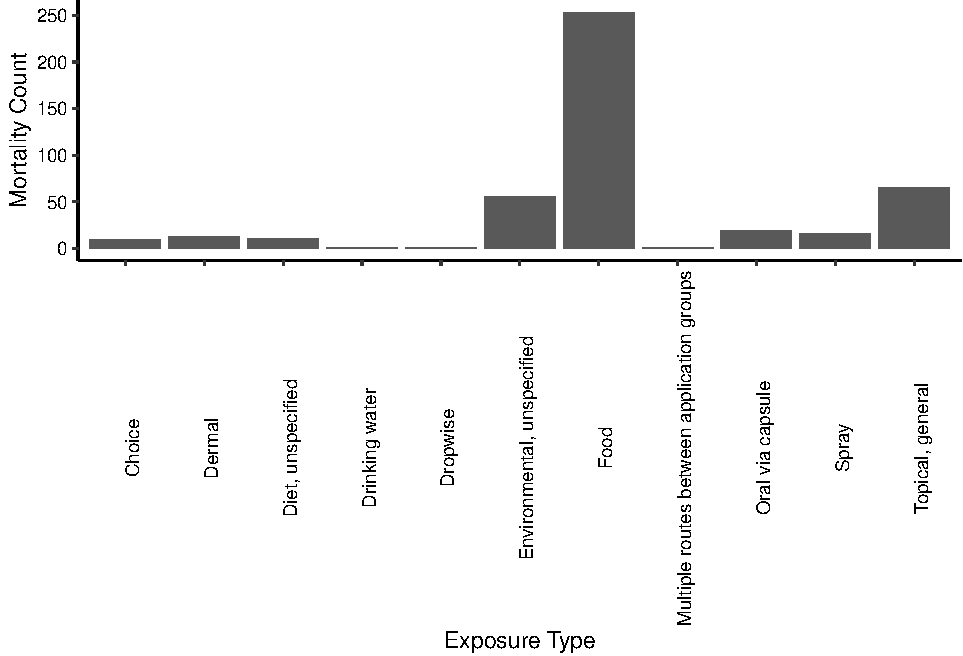
\includegraphics{SamEdit_UpdatedwithModel_files/figure-latex/unnamed-chunk-7-1.pdf}
\caption{Bee Mortality by Exposure Type}
\end{figure}

\begin{verbatim}
##                                         Choice 
##                                             10 
##                                         Dermal 
##                                             13 
##                              Diet, unspecified 
##                                             11 
##                               Dipped or soaked 
##                                              0 
##                             Direct application 
##                                              0 
##                                 Drinking water 
##                                              1 
##                                       Dropwise 
##                                              1 
##                     Environmental, unspecified 
##                                             56 
##                                    Filmcoating 
##                                              0 
##                                   Foliar spray 
##                                              0 
##                                           Food 
##                                            253 
##                                Ground granular 
##                                              0 
##                                   Ground spray 
##                                              0 
##                                  Growth medium 
##                                              0 
##                                     Hand spray 
##                                              0 
##                                      Immersion 
##                                              0 
##                                         Misted 
##                                              0 
##     Multiple routes between application groups 
##                                              1 
## Multiple routes within environmental exposures 
##                                              0 
##                               Oral via capsule 
##                                             19 
##                                Present in soil 
##                                              0 
##                                          Spray 
##                                             16 
##                               Topical, general 
##                                             65 
##                                        Watered 
##                                              0
\end{verbatim}

\begin{verbatim}
##                                         Choice 
##                                             27 
##                                         Dermal 
##                                             66 
##                              Diet, unspecified 
##                                             22 
##                               Dipped or soaked 
##                                              0 
##                             Direct application 
##                                              2 
##                                 Drinking water 
##                                              1 
##                                       Dropwise 
##                                              1 
##                     Environmental, unspecified 
##                                            140 
##                                    Filmcoating 
##                                              0 
##                                   Foliar spray 
##                                              0 
##                                           Food 
##                                            977 
##                                Ground granular 
##                                              5 
##                                   Ground spray 
##                                              0 
##                                  Growth medium 
##                                              0 
##                                     Hand spray 
##                                              4 
##                                      Immersion 
##                                              0 
##                                         Misted 
##                                              0 
##     Multiple routes between application groups 
##                                              7 
## Multiple routes within environmental exposures 
##                                              0 
##                               Oral via capsule 
##                                             19 
##                                Present in soil 
##                                              0 
##                                          Spray 
##                                             37 
##                               Topical, general 
##                                             99 
##                                        Watered 
##                                              0
\end{verbatim}

\begin{figure}
\centering
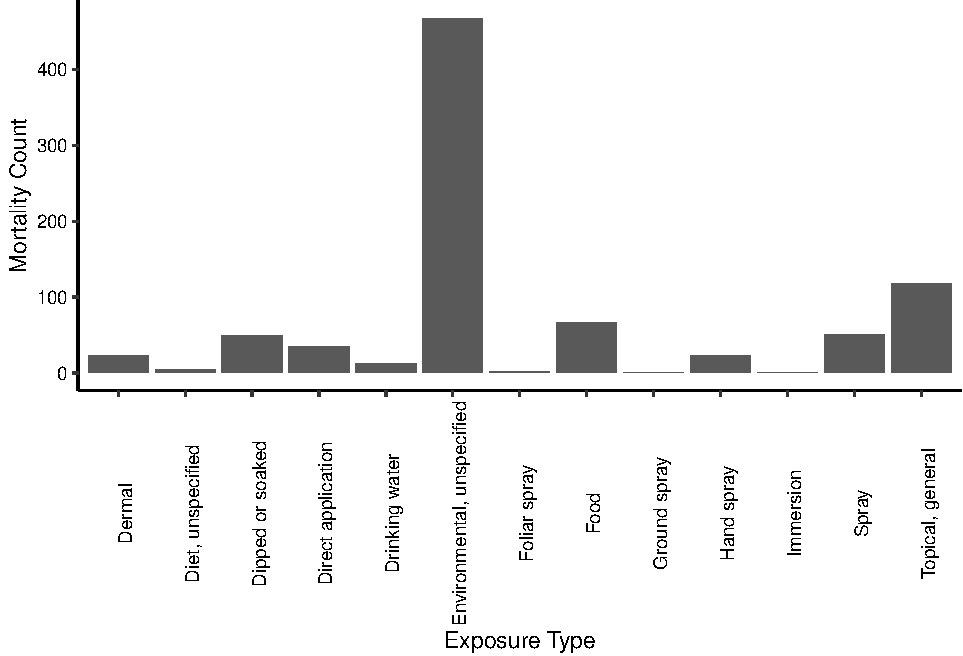
\includegraphics{SamEdit_UpdatedwithModel_files/figure-latex/unnamed-chunk-8-1.pdf}
\caption{Non-bee Mortality by Exposure Type}
\end{figure}

\begin{verbatim}
##                                         Choice 
##                                              0 
##                                         Dermal 
##                                             23 
##                              Diet, unspecified 
##                                              4 
##                               Dipped or soaked 
##                                             49 
##                             Direct application 
##                                             35 
##                                 Drinking water 
##                                             12 
##                                       Dropwise 
##                                              0 
##                     Environmental, unspecified 
##                                            467 
##                                    Filmcoating 
##                                              0 
##                                   Foliar spray 
##                                              2 
##                                           Food 
##                                             67 
##                                Ground granular 
##                                              0 
##                                   Ground spray 
##                                              1 
##                                  Growth medium 
##                                              0 
##                                     Hand spray 
##                                             23 
##                                      Immersion 
##                                              1 
##                                         Misted 
##                                              0 
##     Multiple routes between application groups 
##                                              0 
## Multiple routes within environmental exposures 
##                                              0 
##                               Oral via capsule 
##                                              0 
##                                Present in soil 
##                                              0 
##                                          Spray 
##                                             51 
##                               Topical, general 
##                                            118 
##                                        Watered 
##                                              0
\end{verbatim}

\begin{verbatim}
##                                         Choice 
##                                              0 
##                                         Dermal 
##                                             30 
##                              Diet, unspecified 
##                                              6 
##                               Dipped or soaked 
##                                            109 
##                             Direct application 
##                                            112 
##                                 Drinking water 
##                                             26 
##                                       Dropwise 
##                                              0 
##                     Environmental, unspecified 
##                                           1160 
##                                    Filmcoating 
##                                              1 
##                                   Foliar spray 
##                                            155 
##                                           Food 
##                                            100 
##                                Ground granular 
##                                            210 
##                                   Ground spray 
##                                             64 
##                                  Growth medium 
##                                              0 
##                                     Hand spray 
##                                            148 
##                                      Immersion 
##                                              1 
##                                         Misted 
##                                              8 
##     Multiple routes between application groups 
##                                              0 
## Multiple routes within environmental exposures 
##                                              2 
##                               Oral via capsule 
##                                              0 
##                                Present in soil 
##                                              3 
##                                          Spray 
##                                            254 
##                               Topical, general 
##                                            128 
##                                        Watered 
##                                             12
\end{verbatim}

\begin{figure}
\centering
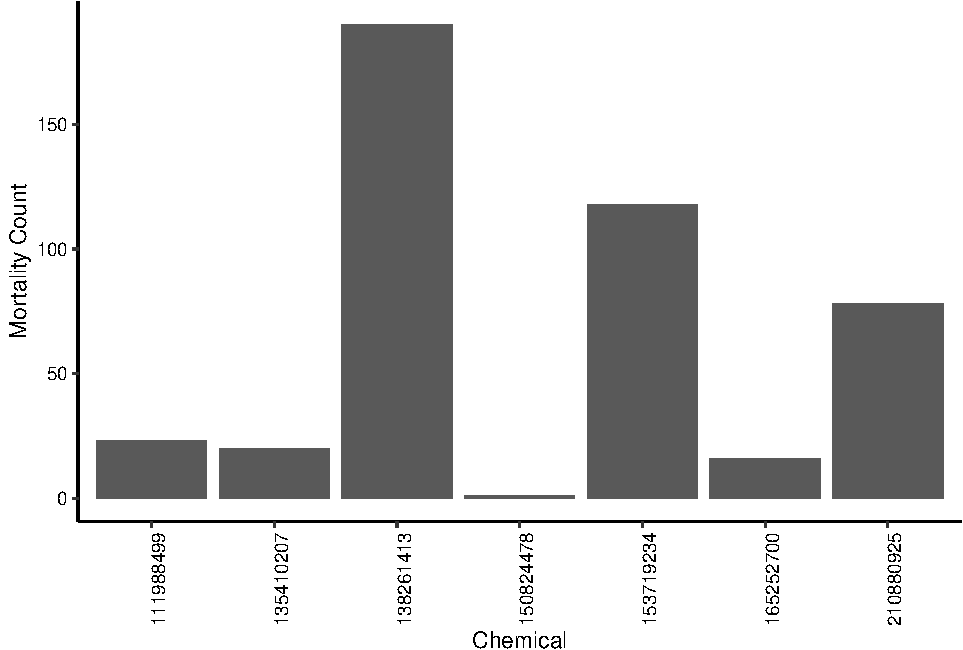
\includegraphics{SamEdit_UpdatedwithModel_files/figure-latex/unnamed-chunk-9-1.pdf}
\caption{Bee Mortality by Chemical}
\end{figure}

\begin{figure}
\centering
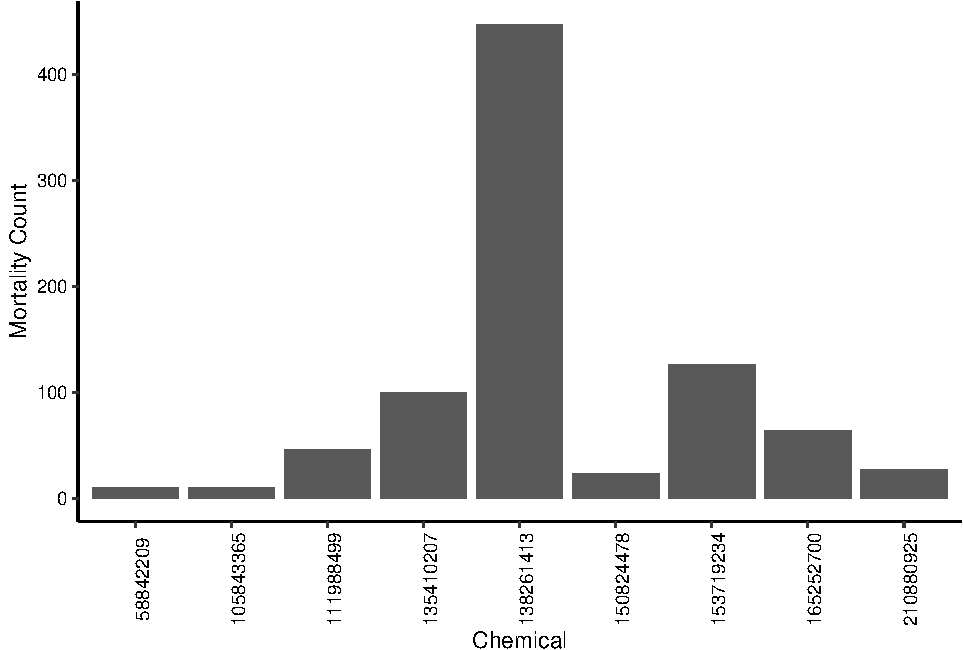
\includegraphics{SamEdit_UpdatedwithModel_files/figure-latex/unnamed-chunk-10-1.pdf}
\caption{Non-bee Mortality by Chemical}
\end{figure}

\newpage

\hypertarget{analysis}{%
\section{Analysis}\label{analysis}}

\hypertarget{question-1-is-there-an-exposure-type-that-has-less-impact-on-bees-than-non-bee-insects}{%
\subsection{Question 1: Is there an exposure type that has less impact
on bees than non-bee
insects?}\label{question-1-is-there-an-exposure-type-that-has-less-impact-on-bees-than-non-bee-insects}}

\begin{longtable}[]{@{}l@{}}
\toprule
x \\
\midrule
\endhead
CAS.Number \\
Chemical.Name \\
Species.Common.Name \\
Organism.Lifestage \\
Organism.Age \\
Exposure.Type \\
Effect \\
Effect.Measurement \\
\bottomrule
\end{longtable}

\hypertarget{question-2-are-there-chemicals-that-have-a-high-mortality-rate-for-non-bee-insects-and-low-rate-for-bees}{%
\subsection{Question 2: Are there chemicals that have a high mortality
rate for non-bee insects and low rate for
bees?}\label{question-2-are-there-chemicals-that-have-a-high-mortality-rate-for-non-bee-insects-and-low-rate-for-bees}}

\newpage

\hypertarget{summary-and-conclusions}{%
\section{Summary and Conclusions}\label{summary-and-conclusions}}

\newpage

\hypertarget{references}{%
\section{References}\label{references}}

\textless add references here if relevant, otherwise delete this
section\textgreater{}

\end{document}
